\documentclass[a4paper,14pt]{extreport}
%\usepackage{pscyr}
\usepackage[T2A]{fontenc}
\usepackage[utf8]{inputenc}
\usepackage[english,russian]{babel}
\usepackage{comment}

\usepackage{amssymb}
%\usepackage{enumerate}  %создание и автоматическая нумерация списков
% \usepackage{amssymb,amsfonts,amsmath,mathtext,cite,enumerate,float}

\usepackage[labelsep=period]{caption} %заменить умолчальное разделение ':' на .
% %'.' в подписях к рисункам и таблицам
\usepackage{graphicx} %разрешить включение PostScript-графики
\graphicspath{{ch1_figures/}{ch2_figures/}}
%\usepackage{epstopdf}

\usepackage{geometry} % Меняем поля страницы
\geometry{left=3cm}% левое поле
\geometry{right=1cm}% правое поле
\geometry{top=2cm}% верхнее поле
\geometry{bottom=2cm}% нижнее поле

\makeatletter
%\bibliographystyle{gost71u-utf8}
\bibliographystyle{utf8gost705u}
\renewcommand{\@biblabel}[1]{#1.}

\makeatother

% % Меняем везде перечисления на цифра.цифра
% \renewcommand{\theenumi}{\arabic{enumi}} 
% \renewcommand{\labelenumi}{\arabic{enumi}}
% \renewcommand{\theenumii}{\arabic{enumii}}
% \renewcommand{\labelenumii}{\arabic{enumi}.\arabic{enumii}.}
% \renewcommand{\theenumiii}{\arabic{enumiii}}
% \renewcommand{\labelenumiii}{\arabic{enumi}.\arabic{enumii}.\arabic{enumiii}.}

\righthyphenmin=2 % Минимальное число символов при переносе - 2.

\pagestyle{plain}
\frenchspacing

\usepackage{cite}
\renewcommand{\baselinestretch}{1.24} % увеличенный межстрочный интервал
\usepackage{indentfirst} %отступ в начале параграфа
% \usepackage{showkeys} %подписи к меткам
\usepackage{amsmath} % мат.формулы
\usepackage{amssymb} % мат.символы
\usepackage{array} % расширенные функции для оформления таблиц
% \usepackage{natbib} % расширенные функции для оформления таблиц
%\usepackage{epsfig}

\renewcommand{\topfraction}{0.9}
\usepackage{hyperref}

%-----------------------------------------------------------%

\newcommand{\tocsecindent}{\hspace{0mm}}

\makeatletter
\renewcommand*\l@chapter{\@dottedtocline{0}{0em}{1.3em}}
\makeatother

%-----------------------------------------------------------%
%-----------------------------------------------------------%

\let\vaccent=\v % rename builtin command \v{} to \vaccent{}
\renewcommand{\v}[1]{\mathbf{#1}} % for vectors
\newcommand{\gv}[1]{\ensuremath{\mbox{\boldmath$ #1 $}}} 
% for vectors of Greek letters
\newcommand{\uv}[1]{\ensuremath{\mathbf{\hat{#1}}}} % for unit vector
\newcommand{\abs}[1]{\left| #1 \right|} % for absolute value
\newcommand{\avg}[1]{\left< #1 \right>} % for average
\let\underdot=\d % rename builtin command \d{} to \underdot{}
\renewcommand{\d}[2]{\frac{d #1}{d #2}} % for derivatives
\newcommand{\dd}[2]{\frac{d^2 #1}{d #2^2}} % for double derivatives
\newcommand{\pd}[2]{\frac{\partial #1}{\partial #2}} 
\newcommand{\pdone}[2]{\partial #1 / \partial #2} 
% for partial derivatives
\newcommand{\pdd}[2]{\frac{\partial^2 #1}{\partial #2^2}} 
% for double partial derivatives
\newcommand{\pdc}[3]{\left( \frac{\partial #1}{\partial #2}
 \right)_{#3}} % for thermodynamic partial derivatives
\newcommand{\ket}[1]{\left| #1 \right>} % for Dirac bras
\newcommand{\bra}[1]{\left< #1 \right|} % for Dirac kets
\newcommand{\braket}[2]{\left< #1 \vphantom{#2} \right|
 \left. #2 \vphantom{#1} \right>} % for Dirac brackets
\newcommand{\matrixel}[3]{\left< #1 \vphantom{#2#3} \right|
 #2 \left| #3 \vphantom{#1#2} \right>} % for Dirac matrix elements
\newcommand{\grad}[1]{\nabla #1} % for gradient
\let\divsymb=\div % rename builtin command \div to \divsymb
%\renewcommand{\div}[1]{\nabla \cdot #1} % for divergence
%\newcommand{\curl}[1]{\nabla \times #1} % for curl
\let\baraccent=\= % rename builtin command \= to \baraccent
\renewcommand{\=}[1]{\stackrel{#1}{=}} % for putting numbers above =
\renewcommand{\phi}{\varphi}
\def\No{\textnumero}

\def\v{\mathbf{v}}
\def\u{\mathbf{u}}
\def\x{\mathbf{x}}
\def\n{\mathbf{n}}
\def\V{\mathbf{V}}
\def\U{\mathbf{U}}
\def\F{\mathbf{F}}
\def\n{\mathbf{n}}
\def\c{\mathbf{c}}
\def\p{\mathbf{p}}
\def\d{\partial}
\def\om{\ensuremath{\mbox{\boldmath$\omega$}}} 
\def\Om{\ensuremath{\mbox{\boldmath$\Omega$}}} 
\def\rot{\mathop{}\!\operatorname{rot}}
\def\div{\mathop{}\!\operatorname{div}}
%\def\grad{\mathop{}\!\operatorname{grad}}
\def\grad{\nabla}
%\def\Laplace{\mathop{}\!\mathbin\bigtriangleup}
\def\Laplace{\mathop{}\!\Delta}
\def\Re{\operatorname{Re}}
%\def\i{\uv{i}}

\begin{document}

\begin{titlepage}
\newpage

%\pagestyle{plain} \thispagestyle{empty}

\begin{center}
{\bf МОСКОВСКИЙ ГОСУДАРСТВЕННЫЙ УНИВЕРСИТЕТ} \\[3pt]
{\bf имени М.В. ЛОМОНОСОВА} \\[3pt]
\begin{tabular}{p{\textwidth}}
\hline {} \\[-14pt]
\end{tabular}
МЕХАНИКО-МАТЕМАТИЧЕСКИЙ ФАКУЛЬТЕТ \\[40pt]
\end{center}

\begin{flushright}
{\it На правах рукописи}\\
УДК 532.517.3: 532.542.3\\[50pt]
\end{flushright}

\begin{center}
{\bf Пиманов Владимир Олегович} \\[30pt]
{\bf ЧИСЛЕННОЕ ИССЛЕДОВАНИЕ ЛОКАЛИЗОВАННЫХ} \\ 
{\bf ТУРБУЛЕНТНЫХ СТРУКТУР В ТРУБАХ} \\[30pt]
{\it 01.02.05 -- механика жидкости, газа и плазмы} \\[30pt]
Диссертация на соискание ученой степени \\
кандидата физико-математических наук \\[30mm]
\hfill\parbox[t]{80mm}{Научный руководитель: \\ д.ф.-м.н., проф. Н.В.~Никитин} \\[5cm]
Москва -- 2017
\end{center}

\end{titlepage}


\setcounter{page}{2}
\tableofcontents

%\chapter{Введение}








Возможным объяснением может быть то, что скорость жидкости падает после того, как в ней возникает турбулентноть, число Рейнольдса падает, и она не распространяется. 

\chapter{Введение}


Цикл самоподдержания пристенной трубулнетности связывают с когерентными стурктурами в буерном слое, наблдаемыми как в экспериментах \cite{kline1967structure}, так и в численных расчетах. Они представляют собой полосы повыешнной и пониженной скорости, вытянутые около стенки вдоль поткоа. Счиатется что они возникают за счет конвекции в нормальной к основному потоку плосоксти, там где медленная жидкость перемещаюется ближе к стенке трубы. 


1995 год: Пристанные структуры самовоспроизводятся. Одни умирают, порождая новые. Основные структуры около стенки - это полосы повышенной и пониженной скорости и продольные вихри. Расстояние между ними -- Kline1967, SmithMetzler1983, Kim1987). После многочисленных исследований кинематика когерентных структур хорошо описана (e.g. Kline et al. 1967; Robinson 1991). но механизмы скрыты, и характеристика не предсказать. 

Direct examination of the flow dynamics in a fully turbulent flow is complicated by the random distribution of the coherent structures in space and time, by the fact that no two realizations of a structure are identical, and by the presence of additional structures (‘debris’) which may not be necessary components of the regeneration process.

Цель ученых упростить задачу так, чтобы остались только существенные её особенности. 

JiminezMoin (1991) --- Численное исследование течения в канале 2000 < Re < 5000. --- и турбулентные законы воспроизвели, и видели полосы, вихри. 
SendstadMoin (1992) --- Тоже считали пристенные структуры. 
Aubry et al. (1988) --- подход динамических систем для исследования продольных вихрей. Как и турбулентность, вихри демонстрируют перемежаемость. Только наблюдение, никаких объяснений. 

Jang, Benney, Gran (1986) --- первая попытка объяснить происхождение пристенных полос. ‘direct resonance’ theory

Waleffe, Kim, Hamilton (1993) --- эта теория не работает. Более того, не один из исследованных ими линейных механизмов не может объяснить расстояние между полосами. 

Butler, Farrell (1993) --- оптимальные возмущения дают полосы. Есть противоречия с другими авторами. 

Jimknez, Moin (1991) --- Турбулентность пропадает, если ширина расчетной области меньше 100 юнитов --- ширины между полосами. Полосы --- важная деталь турбулентности. Waleffe et al. (1993) --- Re лучше вводить через трансверсальную ширину канала; тогда 100 -- критическое число. Это верно для плоского канала, трубы, и еще каких-то штук. 

Jimknez (1994) --- модель течения, воспроизводящая ЦСПТ. Sreenivasan (1988) -- другая, на основе идеи Coles (1978) --- неустойчивость Гетлера (центрифугальная). (Craik, Leibovich 1976) --- похожая неустойчивость. Langmuir circulations --- разработка этой неустойчивости применительно к продольным вихрям, возникающем в ветре на поверхности океана! Craik (1982)

В этой работе течение Куэтта (как у Ньютона). Конец введения. 

Формирование полос за счет продольных вихрей --- Bakewell \& Lumley 1967; Blackwelder \& Eckelmann 1979; Landahl 1980. 

Streak breakdown --- Kim, Kline \& Reynolds 1971; Swearingen \& Blackwelder 1987

Jimhez \& Moin (1991) --- Механизм генерации продольных вихрей: поперечные вихри поворачиваются так, что приобретают нормальную компоненту, затем нормальные вихри поворачивают поперечные так, что они приобретают продольную компоненту. Sendstad \&  Moin (1992) --- причина тоже наклон вихрей. В этом исследовании не так. 

Sendstad \& Moin (1992) --- выделили слагаемое $ - (\partial w / \partial x) (\partial u / \partial y)$, ответственное за генерацию продольных вихрей. Потом листы завихренности сворачиваются в сингулярные вихри. В этой статье говорят, что это слагаемое не работает, так как не дает стационарного вклада. Гетлера неустойчивость тоже не работает. 

Продольные вихри производит нелинейное взаимодействие альфа мод. 
Есть картинка цикла самоподдержания. Выводы --- это цикл. Разнесен во времени. Как-будто нашли нужно слагаемое, но не поняли этого. 

2003 Кавахара \cite{kawahara2003linear}: 

(Kline et al. 1967) --- полосы описал. (Stretch 1990; Jiménez \& Moin 1991; Jeong et al. 1997) --- вихри возникают по бокам от полосы замедления в шахмотном порядке. (Jiménez 1994; Hamilton, Kim \& Waleffe 1995; Waleffe 1997; Kawahara \& Kida 2001) --- Цикл самоподдержания. Panton (1997) --- обзор таких работ --- нет в сети. (Kline et al. 1967, Bakewell \& Lumley 1967) --- полосы производят продольные вихри. (Orlandi \& Jiménez 1994) --- полосы сохдают существенную часть трения на стенке. 

Механизмы генерации продольных вихрей: Jiménez \& Moin (1991) --- они возникают из-за растяжения вихрей(каких?). (Sreenivasan 1988) --- это эффект внешнего потока. (Brooke \& Hanratty 1993) --- эффект прилипания на стенке. Jiménez \& Pinelli (1999) --- полосы необходимы для их возникновнеия. 

Hamilton et al. (1995) --- нашел, что полоса линейно неустойчива (синусоидально), нелинейное трехмерное взаимодействие пульсаций ведет к вихрям. (Waleffe 1997) --- синусоидальная неустойчивость ведет к вихрям?. Вихри нужны только для предотвращения затухания плос за счет вязкости (Itano \& Toh 2001). 

Waleffe (1995, 1997) and Waleffe \& Kim (1997) --- неустойчивость полос из-за точкиперегиба между полосами повышенной и пониженной скорости. Swearingen \& Blackwelder (1987) -- перложен такой тип неустойчивости. Hall \& Horseman (1991) --- другая неустойчивость, между полосой замедления и стенкой, наверное. Важны обе. Обзор здесь Reddy et al. (1998). (Jiménez 1994) --- возникающие вихри нормальны к стенке, но они изгибаются и растягиваются так, что производят продольные. (wake-like mechanism)

Schoppa \& Hussain (1997, 1998) --- продольные вихри возникают еще на стадии линейного роста пульсаций на полосе. Неустойчивость похожа на неустойчивость плоского слоя смешения. Какие-то вихри сприваются. (Schoppa, Hussain \& Metcalfe 1995) --- предположение, что механизм как в слое смешения. (Schoppa 2000; Schoppa \& Hussain 2002) --- неустойчивость полос может быть приближена взволнованным в трансверсальном направлении слоем смешения. Приведены сравнения собственных функций в этом случае с наблюдаемыми. 

Kawahara et al. (1998) --- какая-то модель гладкая течеяни, которую он иследует. Schoppa \& Hussain (1997) --- похожая. Нашли три механизма неустойчивости. 

Schoppa \& Hussain (2002) --- исследовали зависимость скорости роста возмущений от длины волны и амплитуды полос. Затем изсследовали влияние оптимальной волны на полосы. 

(see Schoppa \& Hussain 1997) --- механимы связаны с точкой перегиба а значет не связаны с вязкостью. 

(Moore 1979; Cowley, Baker \& Tanveer 1999). --- скорость роста возмущений на слое смешения тем выше, чем короче их длина. За конечное время сингулярность. 

Ничего не понятно.. 

Schoppa 2002: 

Картинка полос. 

(Townsend 1956; Kline et al. 1967; Kovasz-nay, Kibens \& Blackwelder 1970; Cantwell 1981; Panton 1997) --- пристенные стурктуры. (e.g. Kim, Moin \& Moser 1987). --- доминирующая роль полос в пристенном трении. (Adrian, Meinhart \& Tomkins 1999) --- во внешнем потоке тоже есть структуры. (Jimenez \& Pinelli 1999) --- внешний слой сам по себе, (e.g. Kline et al. 1967) согласен. (e.g. Rao, Narasimha \& Narayanan 1971) --- противоположное мнение, что они связаны. (Jeong \& Hussain 1992; Jeong et al. 1997 (ited by 563)) --- подель цикла самоподержания воспроихводит особенности пристенного течения. 

kawahara2001periodic --- механизм самоподдержания, не только бегущие волны, но и периодические решения воспроихводят цикл. Продолжение темы статьи 1995. 

\section{Обзоры}

\cite{kerswell2005recent} --- обзор Керсвела 2005 год. 

\section{Простые решения}

Кавахара \cite{kawahara2012significance} --- обзор найденных к 2012 году решений, и пояснение смысла этой работы. 

\cite{altmeyer2015role} --- добыли очень устойчивую орбиту из турбулентного течения в трубе. 

\cite{budanur2015periodic} --- 

\section{Турбулентность}


\section{Самоподдержание турбулентного порыва}
\cite{duguet2010slug} --- Путь от решения на сепаратрисе к Слагу. А Слаг, как мы теперь знаем, также структура, что и порыв. 


\section{Самоподдержание пристенной турбулентности}
\cite{waleffe1997self, hamilton1995regeneration, waleffe1995hydrodynamic, waleffe1997self, schoppa2002coherent}

\cite{}


\section{Структуры в турбулентном течении}

Наблюдение полос: \cite{smith1983characteristics, schoppa2002coherent, kline1967structure}
\cite{schoppa2002coherent} -- возможно больше, чем просто наблюдение. 
\cite{klebanoff1962three}

\cite{jeong1997coherent, schoppa2002coherent} -- когерентные структуры. 




\chapter{Введение}

\section{Актуальность}



Изучение закономерностей движения жидкостей и газов в трубах имеет большое значение как с практической, так и теоретической точки зрения. Известно, что при небольших скоростях жидкость в трубах движется ламинарным образом. Такое движение хорошо организовано. Ламинарное течение, устанавливающееся на удалении от входа в трубу, имеет аналитическое представление и называется течением Пуазейля. Частицы жидкости в течении Пуазелйя двигаются по прямым линиям, параллельным оси трубы. Профиль скорости в течении Пуазейля имеет форму параболы. 

По мере увеличения скорости жидкости режим течения сменяется на турбулентный, характеризующийся беспорядочными пульсациями скорости, давления, и других характеристик движения. 


Турбулентность можно отнести к важнейшим из нерешенных задач классической физики и современной науки в целом. Турбулентное движение жидкостей и газов характеризуется резким нерегулярным изменением скорости, давления и других характеристик течения в пространстве и во времени. Турбулентные течения наблюдаются повсеместно, например, в таких технических устройствах, как двигатели внутреннего сгорания или реактивные двигатели, высокоскоростной транспорт, трубопроводные системы. Формирование климата Земли, эволюция звезд и галактик тоже являются сугубо турбулентными процессами. Уравнения, описывающие движение жидкости, известны уже более 150 лет, однако современный математический аппарат не позволяет найти ни их решения, соответствующие турбулентному движению, ни более общие интегральные характеристики таких решений. В частности, величина трения между жидкостью и твердой стенкой может быть получена только из обобщения экспериментальных данных, но не из уравнений движения. Принципиально новые возможности исследования турбулентности открыло развитие вычислительной техники. Численный эксперимент позволяет получить полную информацию о течении --- параметры движения в каждой точке пространства в каждый момент времени. Тем не менее, сегодня нет понимания, каким именно образом движется жидкость в турбулентном потоке, на какие особенности следует обращать внимание при его описании, каким образом можно влиять на это движение. 


Одной из наиболее простых и в тоже время физически реализуемых постановок задачи, в которой наблюдается турбулентность, является движение жидкости в прямой трубе круглого сечения. Исследованию такого течения посвящена пионерская работа Осборна Рейнольдса, в которой в частности был обнаружен безразмерный параметр, определяющий характер течения в трубе, называемый числом Рейнольдса. 

Характер течения определяется единственным безразмерным параметром, числом Рейнольдса (Re), оно пропорционально средней скорости течения. Легко себе представить режим, при котором каждая частица жидкости движется по прямой вдоль трубы. Такой режим наблюдается при небольших числах Рейнольдса и называется ламинарным. По мере увеличения числа Рейнольдса в некоторый момент происходит переход к турбулентности, при этом многократно возрастает трение, которое необходимо преодолеть при прокачивании жидкости через трубу, увеличивается скорость перемешивания и скорость теплопереноса в жидкости, что важно, например, в задачах теплоотвода. Отдельный интерес представляет механизм самоподдержания турбулентности, не позволяющий вернуться к ламинарному течению.При больших числах Рейнольдса турбулентность заполняет всю трубу, в то время как при переходных значениях числа Рейнольдса ламинарный и турбулентный режимы течения сосуществуют. Формируются турбулентные порывы -- локализованные турбулентные структуры, отделенные друг от друга ламинарным потоком [1] (см. Рис. 1). Турбулентные порывы сносятся вниз по потоку примерно со средней скоростью течения , сохраняя при этом свою форму и пространственную протяженность. В длину порыв составляет несколько десятков диаметров трубы. Порыв является удобным объектом для исследования, так как в локальной форме в нем заключен механизм самоподдержания турбулентности. Более того, есть основания полагать, что сплошная турбулентность может быть представлена, как совокупность конкурирующих друг с другом порывов.

Изучению порывов посвящено большое количество работ, но до сих пор не известны как механизмы, приводящие к пространственной локализации, так и причины, определяющие скорость сноса порыва. Исследование осложнено присутствием беспорядочных пульсаций, на фоне которых теряется внутренняя структура турбулентности. Приблизиться к пониманию порыва позволяет анализ найденного в 2013 году [2] уникального решения уравнений Навье-Стокса. В фазовом пространстве это решение принадлежит сепаратрисе -- границе, отделяющей области притяжения ламинарного и турбулентного режимов. Это решение оказывается локализованным в пространстве и ухватывает основные особенности турбулентного порыва, но имеет более простую форму и, что важно, является периодическим по времени в системе отсчета, движущейся вместе с порывом (см. Рис. 2). Такое решение неустойчиво и не может быть воспроизведено в эксперименте, но численно его можно найти. Периодичность по времени позволяет провести его детальное исследование. 

В своей работе [3] мы численно воспроизвели как турбулентный порыв, так и решение на сепаратрисе. Расчеты проводились с использованием ресурсов суперкомпьютерного комплекса МГУ. При помощи метода Ньютона для решения нелинейных систем уравнений удалось найти и другие периодические решения, продлевая решение на сепаратрисе в пространстве параметров. На рис. 3 изображена зависимость скорости сноса и периода по времени от числа Рейнольдса. Решение на сепаратрисе оказывается удобным объектом для демонстрации механизма самоподдержания турбулентности. В предельно простом виде его можно сформулировать следующим образом. Решение на сепаратрисе содержит полосы повышенной и пониженной скорости, вытянутые вдоль стенки трубы вверх по потоку (см. Рис. 2). Эти полосы оказываются неустойчивыми, и на них рождается волна, бегущая вниз по порыву с увеличением амплитуды. Через нелинейное взаимодействие волна поддерживает существование полос. Этот механизм, вероятно, является более общим, так как подобные полосы можно выделить не только в турбулентном порыве, но и во многих других пристенных течениях.


\section{Цели работы}

Цель настоящей работы --- изучение локализованных турбулентных структур, возникающих в трубах круглого сечения, в частности, выявление их механизма самоподдержания. 

\section{Метод исследования и достоверность результатов}

В работе исследуются закономерности турбулентного движения жидкости в круглой трубе и в некоторых других геометриях. Течение жидкости воспроизводится численно путем решения уравнений Навье-Стокса для несжимаемой жидкости. Численный метод совмещает конечно-разностную аппроксимацию по пространственным переменным и полу-неявный метод Рунге-Кутты третьего порядки для интегрирования по времени. 

Возможность адекватного воспроизведение характеристик турбулентного течения в расчетах неоднократно продемонстрирована в большом числе работ. В частности, сравнение результатов расчета турбулентного поля скорости при $\Re = ???$ в круглой трубе с результатами эксперимента представлена здесь. В работе приведены результаты численного расчета турублентных порывов, изучению которых посвящена данная работа. То, что турбулентные порывы могут быть воспроизведены в идеализированной постановке, исключающей неровности стенки или неоднородность потока на входе, доказывает, что свойство локализации является внутренним свойством турбуленности и уранений  Навье-Стокса. 


В последние годы акцент в изучении механизма самоподдержания турбулентности в пристенных течениях смещается от лабораторного эксперимента в сторону эксперимента вычислительного, основанного на численном решении уравнений Навье--Стокса. Турбулентные порывы впервые были рассчитаны в [4], где было показано, что пространственная локализация является внутренним свойством решений уравнений Навье--Стокса при переходных числах Рейнольдса, а не является следствием специальных начальных условий. 

\section{Обзор литературы}

	\subsection{Переход к турбулентности в круглых трубах}

В качестве наиболее простого и в тоже время содержательного с практической точки зрения случая, в котором наблюдается турбулентность, можно выделить движение жидкости в прямых трубах круглого сечения, когда жидкость заполняет все пространство внутри трубы. Известно, что турбулентный режим течения в трубах устанавливается только если скорость потока достаточно велика, при малых скоростях реализуется ламинарное течение. Классическим считается результат Осборна Рейнольдса, опубликованный в 1883 году \cite{Reynolds1883}, согласно которому характер течения жидкости определяется безразмерной комбинацией параметров, называемой числом Рейнольдса. Если число Рейнольдса $\Re = RU/\nu$, вычисленное по максимальной скорости $U$, радиусу трубы $R$, и кинематической вязкости $\nu$, ниже критического значения, близкого к $2000$, то реализуется ламинарный режим течения. При больших $\Re$, как правило, течение оказывается турбулентным. 

Стоит отметить, что в лабораторных условиях, снижая уровень возмущений в потоке и организуя плавный вход жидкости в трубу, можно сохранить течения ламинарным при числах Рейнольдса $\Re \sim 10^4$ и больших \cite{Wygnanski1973, Darbyshire1995, vanDoorne2009}, значительно превышающих критическое значение. Это связано с тем, что турбулентность в трубах возникает жестким образом, без потери ламинарным течением устойчивости к малым возмущениям. Переход к турбулентности вызывают возмущения некоторой достаточно большой амплитуды \cite{Grossmann2000}, присутствующие в потоке. Следуя \cite{Darbyshire1995, Hof2003, Peixinho2007, Mellibovsky2009critical}, пороговое значение амплитуды возмущения, способного вызвать переход к турбулентности, асимптотически уменьшается по мере увеличения числа Рейнольдса по закону $\Re^{-\alpha}$, где $\alpha$ принимает значения от 1 до 2 в зависимости от формы возмущения. Таким образом, с увеличением $\Re$ сохранить течение ламинарным становится все сложнее. 

То обстоятельство, что турбулентность в трубах может существовать несмотря на линейную устойчивость ламинарной формы течения, позволяет говорить о механизме самоподдержания турбулентности, поддерживающем в потоке определенный уровень пульсаций. В случае отсутствия такого механизма амплитуда турбулентных пульсаций будет снижаться за счет вязкости. Когда её величина окажется ниже некоторого критического значения, в потоке установится ламинарный режим течения в силу его линейной устойчивости. На практике наблюдается обратная картина, при достаточно больших значениях $\Re$ турбулентность однажды возникнув продолжает свое существование неограниченно долго и вернуть поток в ламинарное состояние не представляется возможным. 

Обзоры, посвященные ламинарно-турбулентному переходу в трубах, приведены в работах \cite{Kerswell2005, Manneville2016, Kreilos2014, Barkley2016}. 


	\subsection{Локализованные турбулентные структуры}

Осборн Рейнольдс также отметил \cite{Reynolds1883}, что турбулентность в трубах первоначально проявляется перемежающимся образом, когда участки возмущенного и спокойного движения следуют вдоль трубы друг за другом, практически не меняя своей протяженности. На тот момент причина пространственной локализации турбулентности установлена не была. Позднее был выполнен ряд подробных экспериментальных исследований \cite{Lindgren1969, Wygnanski1973, Wygnanski1975, Bandyopadhyay1986, Darbyshire1995, vanDoorne2009}. 
Было установлено, что в разных условиях могут возникать структуры заметно разных типов.

Структуры первого типа --- {\it турбулентные порывы} (turbulent puffs) --- появляются при сильной возмущенности потока на входе в трубу в диапазоне $2000<\Re<2700$. Порывы сносятся вниз по потоку со скоростью, близкой к средней скорости течения, практически не меняя своей протяженности. Длина турбулентного порыва составляет несколько десятков диаметров трубы. Ни в какой другой форме, кроме как в форме порывов, турбулентность в указанном диапазоне числе Рейнольдса в течении длительного времени существовать не может \cite{vanDoorne2009, Moxey2010, Samanta2011}. Даже если возмущения вносятся в поток непрерывно или рассматривается эволюция полностью турбулентного поля скорости, полученного при больших значениях $\Re$, при переходных значениях $\Re$ формируются отдельные области фиксированной длины, разделенные ламинарным течением --- турбулентные порывы. Форма порыва не зависит от начального возмущения, но оно может влиять на их количество и расположение вдоль трубы. Если порывов несколько, они могут быть расположены в трубе нерегулярно, однако расстояние между ними не может быть ниже некоторого минимально значения \cite{Samanta2011}, что отражает тенденцию турбулентности к локализации. В работе \cite{Wygnanski1975} установлено, что при $\Re<2100$ турбулентные порывы подвержены спонтанному исчезновению, а при $\Re>2300$ возможно деление порыва на два следующих друг за другом. Введено понятие {\it равновесного порыва}, характеристики которого не меняются по мере его продвижения вдоль трубы. Согласно \cite{Wygnanski1975} это наблюдается при $2100\leqslant \Re \leqslant 2300$. 

Другой тип локализованных турбулентных структур --- {\it турбулентные пробки} ("turbulent slugs") --- появляются при б\'{о}льших числах Рейнольдса $\Re>3200$ только когда возмущенность потока на входе недостаточна для непосредственного возникновения турбулентности. Турбулентные пробки, двигаясь вниз по трубе, увеличивают свою протяженность, вовлекая в турбулентное движение окружающую жидкость на переднем и заднем фронтах. По мере того, как соседние локализованные структуры нагоняют друг друга, сливаясь вместе, происходит переход к сплошной турбулентности. Непосредственный интерес представляет скорость распространения турбулентной фракции в потоке. Описанию скорости перемещения и структуры фронтов турбулентной пробки посвящены работы \cite{Lindgren1969, Wygnanski1973, Nishi2008, Duguet2010, Barkley2015}. Было установлено, в частности, что турбулентность, по крайней мере до $\Re = 10^5$, не распространяется вверх по течению, то есть скорость заднего фронта положительна в системе отсчета, связанной с трубой, \cite{Wygnanski1973}. 

В работах \cite{Moxey2010, Barkley2015, Song2017} было выполнено подробное исследование динамики фронтом, возникающих на границе областей, занятых ламинарным и турбулентным движением. Было показано, что задний фронт турбулентной пробки качественно не отличим от заднего фронта турбулентного порыва. Он имеет ярко выраженную форму, скорость жидкости вблизи оси трубы падает на нем скачком. По мере увеличения $\Re$, при переходе от динамики турбулентного порыва к турбулентной пробке, скорость заднего фронта плавно снижается. В тоже время, передний фронт претерпевает ряд качественных изменений. При $\Re < 2250$, когда турбулентность представлена турбулентным порывами, скорость переднего фронта совпадает со скорость заднего. При больших $\Re$ передний фронт приобретает собственную скорость, которая возрастает по мере увеличения $\Re$. При $2600 < \Re < 3200$ происходит изменение формы переднего фронта. При меньших значениях $\Re$ он размыт. При б\'{о}льших $\Re$ передний фронт приобретает ярко выраженную форму, повторяющую форму заднего фронта. Стоит отметить, что, хотя уже при $\Re > 2250$ средняя скорость переднего фронта превышает среднюю скорость заднего, и области, в которых наблюдается турбулентное течение, расширяются, в потоке не формируется протяженных турбулентных структур вплоть до $\Re = 3000$. Можно заключить, что турбулентные порывы и турбулентные пробки являются формами одного и того же. 

В работах \cite{Barkley2015, Barkley2016} была предложена модель течения в трубах, воспроизводящая динамику локализованных турбулентных структур. Модель оперирует двумя параметрами, наполненностью среднего профиля скорости и уровнем турбулентных пульсаций, как функциями продольной скоординаты и времени. 

В последние годы было выполнено несколько подробных экспериментальных и численных исследований характеристик и свойств турбулентных порывов [4---10]. Установлено, что турбулентный порыв является нестабильным образованием склонным либо к исчезновению либо к делению. С каждой из двух конкурирующих тенденций может быть связано характерное время: среднее время жизни порыва до его исчезновения и среднее время до его разделения. Первое увеличивается с ростом $Re$, второе уменьшается. Согласно точке зрения, сформулированной в [10], значение $Re=Re^*=2040$, при котором происходит смена доминирования тенденций, является точкой статистического фазового перехода и может быть принята в качестве минимального критического числа Рейнольдса в круглой трубе. При $Re<Re^*$ турбулентный порыв скорее исчезнет, чем успеет разделиться, так что возникновение развитого турбулентного течения невозможно. Наоборот, при $Re>Re^*$ порыв скорее успеет разделиться прежде, чем исчезнет, что приводит к развитию незатухающего турбулентного движения.

Турбулентный порыв представляет собой интересный гидродинамический объект, который в некотором отношении можно рассматривать как структурную единицу турбулентности. Можно сформулировать ряд вопросов, касающихся поведения порыва. До конца не понятен механизм, обуславливающий пространственную локализацию и самоподдержание порыва, неясны причины, побуждающие его к делению или затуханию, неизвестны факторы, определяющие его протяженность и скорость перемещения вдоль трубы.

Большинство работ носят описательный характер, но можно выделить несколько, нацеленных на объяснение формы и механизма самоподдержания турбулентного порыва \cite{Duguet2010, Hof2010, Shimizu2009}. В работе \cite{Duguet2010} предложен механизм, объясняющий расширение локализованных турбулентных структур, но они не касаются механизмов их самоподдержания. В работе \cite{Hof2010} механизм самоподдержания турбулентного порыва связывают с точкой перегиба, расположенной на заднем фронте порыва, если рассматривать поле скорости, как функцию радиальной координаты. В непосредственой близости с точкой перегиба в турбулентном порыва резко падает скорость на заднем фронте, и наблюдается резкий скачет кинетической энергии турбулнетных пульсаций. 
Попытка объяснения механизма сапоподдержания турбулентного порыва была предпринята в \cite{Shimizu2009}. В системе отсчета связанной с порывом, пульсации в осевой части трубы сносятся вниз по потоку. Их нелинейное взаимодействие порождает медленно меняющиеся полосчатые структуры, концентрирующиеся в пристенной области трубы, где относительная скорость течения отрицательная. Из-за этого полосчатые структуры отстают от порыва. В хвостовой части порыва в областях расположения полос замедления образуются интенсивные сдвиговые слои с точкой перегиба в профиле скорости, где в силу неустойчивости типа Кельвина--Гельмгольца порождаются мелкомасштабные пульсации, попадающие в приосевую область трубы и сносящиеся вниз по потоку. Так, согласно \cite{Shimizu2009} выглядит цикл самопроизводства турбулентных пульсаций внутри порыва и цикл самоподдержания самой этой структуры.


	\subsection{Пристенные турбулентные структуры} \label{structure_subsection}


Механизм самоподдержания, описанный в \cite{Shimizu2009}, согласуется с представления о механизме самоподдреания сдвиговых течений в целом. 
\begin{comment}
In the vicinity of a wall, turbulent flow is often found to be highly organized as there exist regions, called coherent structures, where the fluid motion is more strongly correlated than in full turbulence. In figure 1.2.1(a) a flow visualization of a turbulent boundary layer is reproduced from Kline et al. (1967), showing alternating regions of low- and high-speed fluid, elongated in the streamwise direction. The spanwise spacing between these so-called streaks is best expressed in wall units, which are based on the wall shear stress τ W = μ∂u/∂y| y=0 q , with μ = νρ the dynamic viscosity + of the fluid. A length scale is defined by l = ν/ τ W /ρ and the spacing is universally observed to be ∼ 100l + (Klebanoff et al., 1962; Kline et al., 1967). Further investigations (see e.g. Blackwelder and Eckelmann, 1979) reveal the existence of downstream vortices, occuring in counter-rotating pairs. Through linear advection, these vortices push fluid from the high-speed free stream towards the wall, thus creating and sustaining a high-speed streak. Vice versa, fluid is pulled from the wall into the free stream, resulting in a low-speed streak; this process of streak 51. Introduction
creation through downstream vortices is termed lift-up effect. Vortices in near-wall turbulence are typically not exactly parallel to the downstream direction but aligend at a small angle. They are furthermore slightly inclined from the wall (Jeong et al., 1997; Schoppa and Hussain, 2002).
In open flows where no boundaries limit the flow in the wall-normal direction, horseshoe or hairpin shaped vortices are commonly observed (Head and Bandyopadhyay, 1981; Robinson, 1991; Adrian et al., 2000; Adrian, 2007). Close to the wall, these structures are similar to a counter-rotating vortex pair, but they are inclined and extend further into the free stream, where they are connected, forming a hairpin shaped structure. The concept goes back more than half a century to Theodorsen (1952), an illustration is reproduced in figure 1.2.1(b). To better understand the dynamical properties of these typical flow structures, simulations are often performed in so-called minimal flow units defined by the fact that turbulence cannot be sustained if any of the dimensions is reduced (Jiménez and Moin, 1991), with some freedom in the definition of sustained turbulence and the ratio of the dimensions. The concept is useful because it allows to extract features of turbulence which are otherwise obfuscated by spatial processes and because a small periodic domain is cheaper in numerical simulations. In such a minimal flow unit, a self-sustaining cycle of near-wall turbulence has been identified (Hamilton et al., 1995; Waleffe, 1997, 2003), connecting the typical flow structures and their instabilities. The cycle starts with a pair of counter-rotating streamwise-aligned vortices, which create a pair of streaks through the lift-up effect. The streaks, initially straight, are linearly unstable to developing a wavy modulation, and the period in which the streaks are created is about as long as the subsequent period during which the instabilities grow. As the modulation becomes too strong, the structures break up, leaving behind a flow with strong downstream variations. The cycle is closed by nonlinear interactions recreating the downstream vortices. This so called self-sustaining process is found in many shear flows and was, for example, observed experimentally by Duriez et al. (2009). It also served as the stimulus for making an analogy between fluid mechanics and magnetohydrodynamic dynamos (Riols et al., 2013). 
\end{comment}

	\subsection{Сдвиговые течения}

This is common for wall-bounded shear flows (Manneville 2015) --- жесткое возбуждение турбулентности



	\subsection{Решение на сепаратрисе}


https://hal.archives-ouvertes.fr/file/index/docid/1021118/filename/S0022112010003435a.pdf

Можно отметить, что течение Пуазейля, соответствующее ламинарному течению, устанавливающемуся на удалении от входа в трубу, устойчиво к малым возмущениям при всех $\Re$, как принято сегодня считать \cite{Kerswell2005}. Линейная устойчивость течения Пуазейля была показана численно до $\Re=10^7$ \cite{Meseguer2003}, а также аналитически для осесимметричных возмущений \cite{Salwen1980}. 

Идеализированная схема, предложенная в [11], выглядит вполне правдоподобно, однако, на наш взгляд, сделанные выводы в должной мере не подкреплены фактическими данными. Реальная динамика порыва сложнее и неопределеннее. Ее изучение осложнено в первую очередь стохастичностью процесса, когда отдельные его фазы следуют друг за другом случайным образом. В этих условиях определенная ясность может быть получена из анализа более простых структур, аппроксимирующих порыв, недавно найденных в [12,13]. Это предельные решения, возникающие на сепаратрисе, разделяющей в фазовом пространстве области притяжения решений, соответствующих ламинарному и турбулентному режимам течения. Такие решения, наследуя ряд качественных характеристик турбулентного порыва, оказываются периодическими по времени в системе отсчета, перемещающейся вдоль трубы с постоянной скоростью. Простота поведения позволяет провести исчерпывающее исследование свойств таких условно периодических решений, которые, как мы полагаем, проясняют определенные детали поведения турбулентного порыва.

\section{Апробация работы}

\section{Благодарности}




\chapter{Метод решения}

\section{Введение}


Представленное в диссертационной работе исследование выполнено методом прямого численного моделирования. 


During the last decades, direct numerical simulations (DNS) have been recognized as a powerful and reliable tool for studying the basic physics of turbulence. 


\section{Математическая постановка задачи}

Рассматривается течение вязкой несжимаемой жидкости в прямой трубе круглого сечения. Жидкость считается однородной --- её плотность $\rho$ и вязкость $\mu$ во всем объеме трубы постоянны. Движение вызывается внешним градиентом давления, направленным вдоль трубы.


Поле скорости $\v(\x,t)$ удовлетворяет уравнению несжимаемости
\begin{equation} \label{eq0}
\nabla \cdot \v = 0.
\end{equation}

Движение жидкости описывается уравнениями Навье-Стокса, которые для несжимаемой жидкости имеют вид
\begin{equation} \label{NSeq_dynamic}
\pd{\v}{t} = - (\v, \nabla) \v - \frac{1}{\rho}\nabla \Pi + \frac{\mu}{\rho} \nabla^2 \v.
\end{equation}
Здесь $\Pi = \Pi(\x,t)$ --- поле давления. Уравнения решаются в цилиндрической системе координат $(x,r,\theta)$, где $x$ --- продольное, $r$ --- радиальное и $\theta$ --- угловое направления, $t$ --- время. 


На твердой стенке трубы радиуса $R$ ставятся условия прилипания
\begin{equation} \label{bc0}
\v = 0 \text{ при } r = R.
\end{equation}
В направлении движения устанавливаются условие периодичности с периодом $L_x$. Давление $\Pi$, непосредственно, периодическим не является. Оно представляется в виде суммы периодической $p$ и линейной вдоль трубы $Dx$ составляющих. Подстановка $\Pi = p + Dx$ в \eqref{NSeq_dynamic} дает уравнение
\begin{equation} \label{NSeq_periodic}
\pd{\v}{t} = - (\v, \nabla) \v - \frac{D}{\rho}\i - \frac{1}{\rho}\nabla p + \frac{\mu}{\rho} \nabla^2 \v.
\end{equation}
Здесь $\i$ -- единичный орт, направленный вдоль трубы. В уравнении \eqref{NSeq_periodic} все переменные удовлетворяют условию периодичности вдоль трубы
\begin{equation} \label{bc1}
[\v, p](x,r,\theta,t) = [\v, p](x+L_x,r,\theta,t).
\end{equation}

Величина $D$ представляет собой внешний градиент давления, которые определяется из условия постоянства расхода жидкости, протекающей через трубу. Постановка задачи может быть легко обобщена на случай наличия внешних потенциальных сил $\F = \nabla U$. За $D$ в этом случае следует обозначить разность внешнего градиента давления и средней вдоль трубы составляющей $F_x$. Не вошедшая в $D$ часть $\F$ потенциальна. Разность периодической вдоль трубы части давления и её потенциала составляет $p$. 

Поставленная задача, определяемая уравнениями \eqref{eq0}, \eqref{bc0}, \eqref{NSeq_periodic}, \eqref{bc1}, имеет единственное решение для каждого начального поля скорости $\v_0(\x)$, удовлетворяющего условию несжимаемости \eqref{eq0}. Известно аналитическое решение задачи, называемое течением Пуазейля, соответствующее ламинарному режиму течения. Оно существует при всех значениях параметров и задается формулой
\begin{equation}
\v = (U (1 - (r / R)^2), 0, 0).
\end{equation}
Здесь величина $U = - D R^2\mu^{-1}/4 $ определяется по градиенту давления $D$ и соответствует максимальной скорости в ламинарном течении, которую оно достигает на оси трубы. Несложно показать, что средняя скорость течения $U_q$, вычисленная как отношение расхода к площади сечения трубы, в этом случае равна $U/2$. 


В работе все вычисления выполняются в безразмерных переменных. В качестве масштабов выступают радиус трубы $R$, максимальная скорость в ламинарном течении $U$ и плотность жидкости $\rho$. Переход к безразмерным единицам измерения, обозначенным штрихами, выполняется по формулам
\begin{equation} \label{dim_less_eqs}
R x' = x,  R r' = r, RU^{-1} t' = t, U\v' = \v , \rho U^2 p' = p, \rho U^2 R^{-1} D' = D, R L'_x = L_x.
\end{equation}

В безразмерных единицах измерения уравнения \eqref{eq0}, \eqref{bc0}, \eqref{NSeq_periodic}, \eqref{bc1} принимают вид (штрихи опущены):
\begin{equation}\label{eq0_Re}
\nabla \cdot \v = 0,
\end{equation}
\begin{equation}\label{NSeq_Re}
\pd{\v}{t} = - (\v, \nabla) \v - \i D - \nabla p + \frac{1}{\Re} \nabla^2 \v,
\end{equation}
\begin{equation}\label{bc0_Re}
\v = 0 \text{ при } r = 1,
\end{equation}
\begin{equation}\label{bc1_Re}
[\v, p](x,r,\theta,t) = [\v, p](x+L_x,r,\theta,t)
\end{equation}
Здесь $\Re = \rho R U / \mu$ --- число Рейнольдса, один из двух параметров системы. Вторым параметром является $L_x$. Величина $D$ подбирается из условия постоянства расхода так, что $U_q = 1/2$ в безразмерных единицах. В случае ламинарного течения она выражается в явном виде: $D = - 4 \Re^{-1}$. Ламинарное течение в безразмерном виде задается более простым выражением 
\begin{equation}
\v = (1 - r^2, 0, 0).
\end{equation}

Многие авторы вводят число Рейнольдса иначе, через расходную скорость $U_q$ и диаметр трубы $D$. Несложно показать, что значение числа Рейнольдса, введенного таким образом, совпадает со значением числа Рейнольдса, введенного выше. Однако, например, единица измерения времени $DU_q^{-1}$ в этом случае увеличивается в 4 раза.

В процессе решения задачи возникает необходимость перехода в подвижную систему координат. Выполняя переход, удобно сохранить в качестве тела, относительно которого определяются скорости, стенки трубы. В этом случае граничные условия и значения скорости не зависят от системы отсчета, но в уравнении движения \eqref{NSeq_Re} возникает новое слагаемое
\begin{equation}\label{NSeq_cf}
\pd{\v}{t} = c_f \pd{\v}{x} - (\v, \nabla) \v - \i D - \nabla p + \frac{1}{\Re} \nabla^2 \v. 
\end{equation}
Возникшее слагаемое отвечает за перенос решения вдоль трубы со скоростью $-c_f$, где $c_f = c_f(t)$ --- скорость перемещения системы координат, может быть функцией времени. Уравнение неразрывности \eqref{eq0_Re} при переходе, выполненном таким образом, не меняется. 


Поставленная задача сформулирована традиционным образом для прямого расчета турбулентных потоков в прямых каналах. В такой постановке удается воспроизводить характеристики течения, устанавливающегося на большом удалении от входа в трубу, решая уравнения лишь в ограниченной расчетной области. Условие периодичности освобождает от необходимости устанавливать условия на входе и выходе из трубы. В тоже время, увеличивая длину периода $L_x$, можно минимизировать влияние этого условия на поток. Для того, чтобы иметь возможность воспроизвести в расчете локализованные турбулентные структуры, необходимо выдирать длину $L_x$ достаточно большой, не менее $40$ диаметров трубы. 


\section{Численный метод}

\begin{comment}
Поставленная задача решается численно конечно-разностным методом \cite{nikitin2006method}. Метод формулируется относительно уравнения движения \eqref{NSeq_Re}, преобразованного к виду 
\begin{equation}\label{NSeq_om}
\pd{\v}{t} = - \i D + \v \times \om - \nabla P - \frac{1}{\Re} \rot \om
\end{equation}
Здесь $\om = \rot \v$ --- вектор завихренности, посчитанный по полю скорости $\v$, $P = p + |\v|^2/2$ --- полное кинематическое давление. Эквивалентность уравнений \eqref{NSeq_Re} и \eqref{NSeq_om} следует из векторных тождеств
\begin{equation*}
-(\v, \nabla) \v = \v \times \rot \v - \nabla |\v|^2/2,
\end{equation*}
\begin{equation*}
\nabla^2 \v = \grad \div \v - \rot \rot \v.
\end{equation*}
\end{comment}

Поставленная задача решается численно конечно-разностным методом \cite{nikitin2006method}, в цилиндрической системе координат $(x,r,\theta)$. Расчетная область в переменных $(x,r,\theta)$ имеет форму параллелепипеда
\begin{equation}
0 < x < L_x, 0 < r < 1, 0 < \theta < 2\pi.
\end{equation}
При решении уравнений в этих переменных необходимо дополнительно установить условия периодичности в направлении $\theta$ и ограниченности решения при $r=0$.

В переменных $(x,r,\theta)$ в расчетной области вводится прямоугольная система координат, однородная в направлениях $x$ и $\theta$. В радиальном направлении вводится растяжение сетки, что позволяет сгустить её вблизи стенки. Во всех расчетах, приведенных ниже, параметр растяжения выбран так, что размер ячейки в радиальном направлении около стенки в 4 раза меньше, чем в центре трубы. 

При дискретизации уравнений применен подход, при котором различные неизвестные определяются в различных точках сетки. Так, давление $p$ относится к центру ячеек. Компоненты вектора скорости $v_k$ относятся к центрам граней, нормальных к направлению $k$. В процессе счета и при анализе решений возникает необходимость вычисления завихренности $\omega$. Компоненты вектора завихренности $\omega_k$ относятся к центрам ребер, параллельных направлению $k$. При таком подходе говорят, что неизвестные определены на смещенных или разнесенных сетках. Он позволяет естественным образом ввести аппроксимацию уравнения второго порядка точности по пространству. 

Пространственная дискретизация введена таким образом, что сохраняется ряд важных консервативных свойств исходной системы. В частности, тождественно равна нулю дивергенция вязких слагаемых в \eqref{NSeq_Re}, что гарантирует, что это слагаемое не производит массы. Также тождественно равна нулю завихренность градиента давления, что обеспечивает отсутствие влияния давления на эволюцию завихренности непосредственно. 

При моделировании турбулентных течений важно аккуратно воспроизводить изменение кинетической энергии системы. Уравнение, описывающее его, возникает в результате скалярного умножения на $\v$ уравнений движения \eqref{NSeq_Re} с последующим суммированием по всей расчетной области. Важным свойством системы является то, что в уравнении Навье-Стокса для несжимаемой жидкости градиент давления и нелинейные слагаемые не производят кинетической энергии, а лишь перераспределяют уже существующую. В конечно-разностной постановке строго выполняются тождества, выражающие этот факт, выполненные при \eqref{eq0_Re}, \eqref{bc0_Re}, \eqref{bc1_Re}
$$
\int_V \v \cdot \nabla p\ d\tau= \int_V \nabla (\v p) d\tau = \int_{\Sigma} p v_n d\sigma = 0, 
$$
$$
\int_V \v \cdot (\v, \nabla) \v\ d\tau = \int_V (\v, \nabla)\frac{|\v|^2}{2}\ d\tau = \int_V \nabla (\v \frac{|\v|^2}{2}) d\tau = \int_{\Sigma} \frac{|\v|^2}{2} v_n d\sigma = 0.
$$
Здесь $V$ --- расчетная область, $\Sigma$ --- её граница, $v_n$ --- нормальная составляющая скорости на границе. Также строго выполняется дискретный аналог уравнения изменения полной кинетической энергии $E$, записанного в следующем виде
\begin{equation} \label{Eeq}
\d{E}{t} = - \frac{1}{2}DV - \frac{1}{\Re} \int_{V} |\omega|^2 d\tau,
\end{equation}
$$
E = \frac{1}{2}\int_{V} |\v|^2 d\tau.
$$
Изменение полной энергии происходит за счет внешнего градиента давления $D$ и вязкой диссипации. 

Интегрирование по времени выполняется полу-неявным методом Рунге-Кутты третьего порядка точности \cite{Nikitin2006Third}. В силу нелинейности оператора Навье-Стокса реализовать полностью неявный метод продвижения по времени затруднительно. Однако наибольшая жесткость системы на достаточно подробных сетках вызвана вязкими слагаемыми. В силу их линейности они могут быть разрешены неявно в то время, как другие слагаемые в операторе Навье-Стокса разрешаются явно. Такой подход позволяет существенно увеличить допустимый временной шаг в сравнении с явными методами. Реализованный алгоритм допускает автоматический выбор шага интегрирования исходя из условия сохранения локальной точности получаемого решения. Таким образом шаг интегрирования автоматически адаптируется к изменением в структуре течения, и не требует явного его задания во время счета. 


На каждом шаге по времени возникает необходимость по известному полю скорости $\v$ определить давление $p$. Для этого необходимо решить уравнение Пуассона, возникающее в результате применения оператора дивергенции к уравнению движения \eqref{NSeq_Re} при условии несжимаемости \eqref{eq0_Re}, имеющее вид
\begin{equation}\label{Peq}
\nabla^2 p = \div \tilde \v,
\end{equation}
$$
\tilde \v = - (\v,\nabla)\v + \frac{1}{\Re}\nabla^2 \v. 
$$
Правая часть уравнения \eqref{Peq} известна. Давление также удовлетворяет условию периодичности в направлениях $x$ и $\theta$. На оси трубы значение давления ограничено. Условие на твердой стенке возникает в результате проектирования уравнения \eqref{NSeq_Re} на направление нормали $n$
$$
\pd{p}{n} = \tilde v_n.
$$


Простая геометрия расчетной области позволяет применять прямые методы решения возникающей линейной системы. Метод решения задачи для давления основан на применении быстрого преобразования Фурье в направлениях $x$ и $r$. В радиальном направлении система решается методом прогонки. Общая сложность решения задачи для давления составляет $O(N \log N)$, где $N$ --- количество ячеек в сетке. Решение задачи для давления составляет основную вычислительную сложность используемого метода. 

\section{Методические расчеты}


Приводимые ниже результаты расчетов в диапазоне $1670\leqslant Re\leqslant 2800$ получены при $L_x=200$ с пространственным разрешением $2048 \times 64 \times 128$ в продольном, радиальном и угловом направлении соответственно. Расчеты на более грубой сетке $1024\times32\times64$ во всех рассмотренных случаях дают результаты совпадающие качественно и близкие количественно.

Стартуя с начальных данных в виде некоторого трехмерного возмущения течения Пуазейля, уравнения Навье--Стокса интегрируются до выхода решения на тот или иной режим. Установление решения, отвечающего турбулентному течению происходит в том случае, когда амплитуда начального возмущения достаточно велика, в противном случае возмущения затухают со временем, и решение в конечном итоге возвращается к ламинарному течению Пуазейля. Турбулентный режим за пределами диапазона переходных чисел Рейнольдса $Re\geqslant3000$ имеет вид статистически стационарного процесса и не зависит от конкретного вида начальных условий, при которых он был получен. Течение при этом однородно в продольном направлении, его статистические характеристики согласуются с имеющимися экспериментальными данными. При $\Re\leqslant2600$ в распределении скорости вдоль трубы появляется неоднородность, которая при $\Re\lesssim2200$ приобретает форму двигающейся вдоль трубы цепочки из нескольких пространственно-локализованных структур, разделенных участками ламинарного течения. Конкретное число получающихся в решении турбулентных структур зависит от начальных условий. Кроме того, как было отмечено выше, это число может меняться в процессе эволюции в результате исчезновения или деления отдельных структур. Получаемые в расчетах пространственно-локализованные турбулентные структуры хорошо согласуются с наблюдаемыми в экспериментах турбулентными порывами, что позволяет нам пользоваться этим их наименованием. Отметим, что турбулентные порывы формируются и на некотором отрезке времени существуют в расчетах и при $Re<2000$, вплоть до $Re=1670$. Однако, в этом случае не только число порывов в пределах расчетной области, но и время их существования является случайной величиной и зависит от конкретных начальных условий. Представленная на фиг.~1 визуализация рассчитанных течений в диапазоне $1680\leqslant Re\leqslant2800$ демонстрирует эволюцию локализованных структур при изменении числа Рейнольдса.






\chapter{Модельный порыв}

\section{Введение} 


В круглой трубе течение Пуазейля устойчиво к малым возмущениям. Для выхода на турбулентное решение, стартуя с возмущенного течения Пуазейля, амплитуда возмущения должна быть достаточно велика. Кроме амплитуды возмущнеия имеет значения также его форма. В частности, любые осесимметричные возмущения течения Пуазейля затухают. Для начального возмущения фиксированной формы можно определить такое значение амплитуды, что решение в процессе эволюции будет оставаться на сепаратрисе, разделяющей в фазовом пространстве области притяжения ламинарного и турбулентного решений. Это решение неустойчиво и при численном интегрировании рано или поздно сваливается в ту или иную сторону --- либо выходит на турбулентный режим, либо возвращается к течению Пуазейля. Тем не менее, варьируя начальную амплитуду возмущения, можно проследить поведение балансирующего на сепаратрисе решения на значительном промежутке времени. Как показано в \cite{Skufca2006}, предельное решение, к которому стремится решение на сепаратрисе, сохраняет некоторые черты турбулентного решения, но при этом как правило обладает более простым поведением во времени. В \cite{Avila2013} обнаружено, что при наложении дополнительных ограничений симметрии предельное решение на сепаратрисе при $Re\sim2000$ качественно близко к турбулентному порыву, но оказывается при этом условно-периодическим по времени, а именно, периодическим в подходящей подвижной системе отсчета. Простота поведения предельного решения на сепаратрисе позволяет провести его исчерпывающее исследование, что на наш взгляд может быть небесполезным для понимания  механизма образования и самоподдержания турбулентных порывов. Мы будем называть решение на сепаратрисе модельным порывом. 

Основные результаты, приведенные в этом разделе, опубликованы в работах автора    \cite{MZG2015, Kazan2015, MZG2017}. 

\section{Метод поиска решения на сепаратрисе}

Следуя \cite{avila2013streamwise}, решение уравнений Навье--Стокса ищется с дополнительными ограничениями диаметральной симметричности и $\pi$-периодичности поля скорости $\u=(u_x,u_r,u_\theta)$ в угловом направлении:
\begin{equation}\label{sym_eq}
(u_x,u_r)(x,r,-\theta,t)=(u_x,u_r)(x,r,\theta,t),\ \ u_\theta(x,r,-\theta,t)=-u_\theta(x,r,\theta,t)
\end{equation}
\begin{equation}\label{per_eq}
(u_x,u_r,u_\theta)(x,r,\theta+\pi,t) = (u_x,u_r,u_\theta)(x,r,\theta,t)
\end{equation}
Здесь $(x,r,\theta)$ --- цилиндрические координаты. Наложение ограничений \eqref{sym_eq}, \eqref{per_eq} упрощает поведение решения в пространстве, делает его более определенным, но важно, что оно остается решением исходной системы. Турбулентные порывы, рассчитанные при $Re=2000$ с учетом и без учета условий \eqref{sym_eq}, \eqref{per_eq} изображены на фиг.~\ref{3D_img} (представлены области пониженной и повышенной на $0.1$ скорости относительно течения Пуазейля). В обоих случаях порыв имеет центральное ядро с пониженной скоростью и систему вытянутых вдоль стенки трубы, чередующихся в угловом направлении полос замедления и ускорения. На симметричном порыве полосы гораздо более структурированы. Их угловое положение не меняется в процессе эволюции: угловые области $\theta=k\pi/2,\ k=0-3$, где в силу \eqref{sym_eq}, \eqref{per_eq} угловая компонента скорости тождественно равна нулю, заняты полосами ускорения, промежуточные области $\theta=\pi/4+k\pi/2$ --- полосами замедления. На порыве без условий симметрии наблюдаются значительные по амплитуде случайные по пространственному расположению флуктуации, разрывающие сплошность полосчатых структур. На симметричном порыве тоже заметна флуктуирующая компонента, которая в этом случае выглядит гораздо более регулярной. Отметим, что несмотря на заметную пространственную регулярность, временн\'{о}е поведение симметричного порыва остается хаотичным.


\begin{figure}[h]
\center{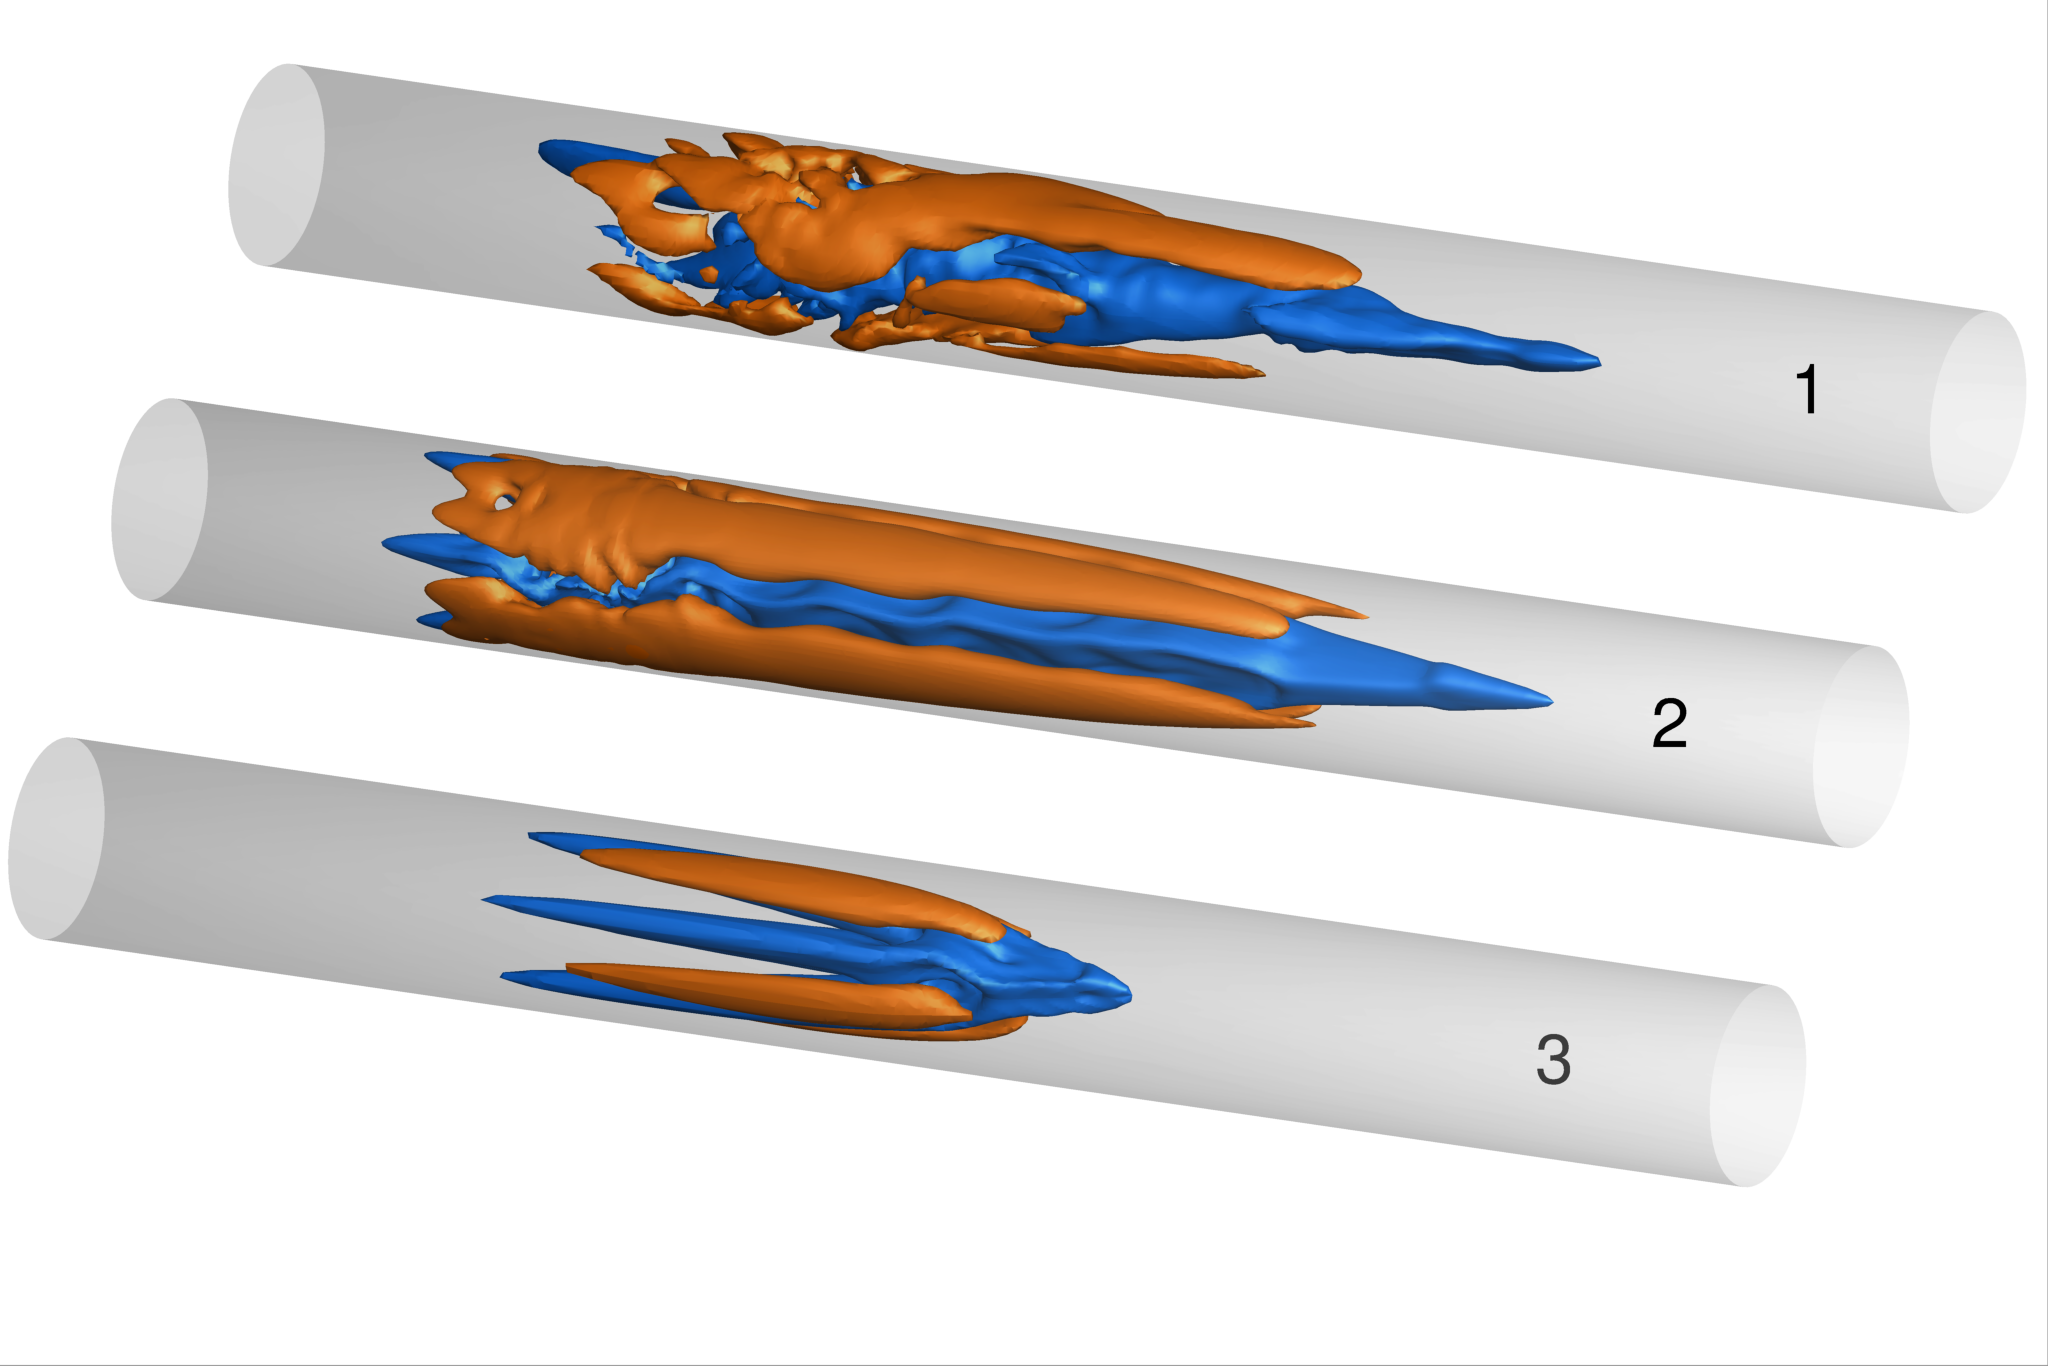
\includegraphics[width=1\linewidth]{3D_cmp.png}}
\caption{Визуализация численных расчетов турбулентных порывов: 1 --- Re = 2000; 2 --- Re = 2000 с учетом \eqref{sym_eq}, \eqref{per_eq}; 3 --- решение на сепаратрисе, Re = 2200. Темным и светлым тоном выделены поверхности скорости –0.1 и + 0.1 относительно скорости течения Пуазейля. Направление потока слева направо.}
\label{3D_img}
\end{figure}

Предельное решение на сепаратрисе рассчитывалось при $Re=2200$. С учетом условий \eqref{sym_eq}, \eqref{per_eq} расчет проводился для четверти объема трубы $0\leqslant\theta\leqslant\pi/2$. Решение на сепаратрисе было найдено на трех сетках. Исходная сетка построена в расчетной области длиной $L_x = 80$ и имеет $512 \times 32 \times  32$ ячеек. Для того, чтобы продемонстрировать, что решение не зависит от длины расчетной области, было также найдено решение при вдвое большем значении $L_x = 160$ на сетке с вдвое большим числом узлов в продольном направлении $1024 \times 32 \times 32$. Для того, чтобы показать сеточную сходимость, решение также было найдено на третьей сетке при исходном значении $L_x=80$ с вдвое большим пространственным разрешением $1024 \times 64 \times 64$. Решения, полученные на каждой из сеток, качественно совпадают и близки количественно, что подтверждает физический характер решения. Решение не зависит от численного метода, так как в работах других авторов решение было найдено другими численнымим метода, в частности спектральным, и наблдается хорошее сходноство характеристик решения. 

Предварительно найденное турбулентное решение $\u_{turb}(\x,t)$ используется в итерационной процедуре отыскания предельного решения на сепаратрисе. Задача решается с начальным условием
\begin{equation*}\label{init}
  \u(\x,t=0) = \u_{Pois}(\x)+\alpha(\u_{turb}(\x,t=t_0) - \u_{Pois}(\x))
\end{equation*}
Здесь $\u_{Pois}=(1-r^2,0,0)$ --- течение Пуазейля, $t_0$ --- некоторый фиксированный момент времени, $\alpha\in[0,1]$ --- скалярный параметр. Значение $\alpha=0$ соответствует нулевому возмущению, и решением при $t>0$ остается течение Пуазейля. Выбирая $\alpha=1$, мы уже в начальный момент времени попадаем на турбулентный режим и остаемся на нем при $t>0$. При промежуточных значениях $\alpha$ происходит стремление решения либо к одному, либо к другому режиму. Применяя метод деления пополам, мы постепенно отыскиваем то значение $\alpha$, при котором решение эволюционирует на сепаратрисе, разделяющей области притяжения двух режимов течения. На фиг.~\ref{bisection_pic} представлены графики $A(t)$ --- среднеквадратичного по всему объему отклонения поля скорости от течения Пуазейля для нескольких значений $\alpha$, демонстрирующие сходимость итерационного процесса. Уточняя значение $\alpha$, мы продлеваем длительность балансирования решения на сепаратрисе.

\begin{figure}[h]
\center{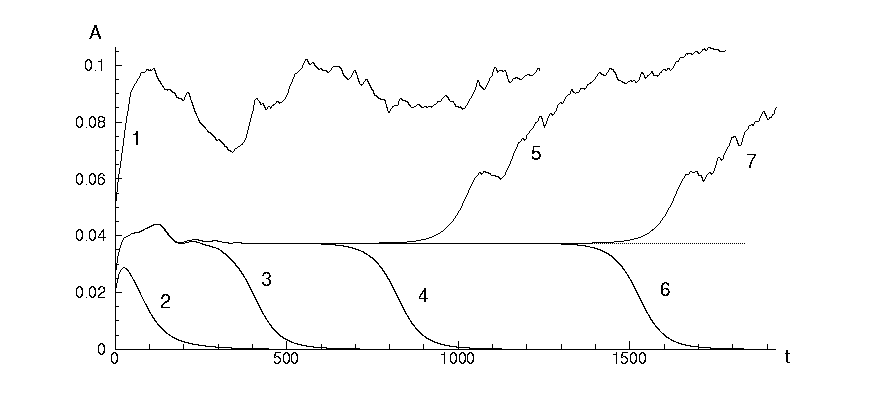
\includegraphics[width=1\linewidth]{bisection.png}}
\caption{Итерационный процесс построения решения на сепаратрисе. 1--7 --- эволюция среднеквадратичной амплитуды возмущений $A(t)$ при уточнении начального
значения.}
\label{bisection_pic}
\end{figure}

В согласии с результатами \cite{Avila2013}, решение на сепаратрисе при $Re=2200$ постепенно выходит на условно периодический режим. Это решение, как и турбулентный порыв, имеет форму локализованой в пространстве структуры, которая сносится вниз по потоку с постоянной скоростью. В подвижной системе отсчета поле скорости в каждой точке испытывает периодические колебания. Для скорости сноса и периода колебаний получены значения $C_f=0.69$ и $T=60$ (в [13] сообщается о $C_f=0.76$ и $T=60$). Сравнение предельного решения на сепаратрисе с турбулентным порывом, представленное на фиг.~\ref{3D_img}, показывает качественное согласие этих решений. Во всех структурах имеются протяженные области ускоренного и замедленного движения, концентрирующиеся в пристенной области трубы. Сохраняется и основная качественная особенность порыва --- медленное понижение осевой скорости на переднем фронте и более резкое восстановление на заднем. Скорость на оси трубы изобрадена на фиг.~\ref{ucl_cmp_img}. 

\begin{figure}[h]
\center{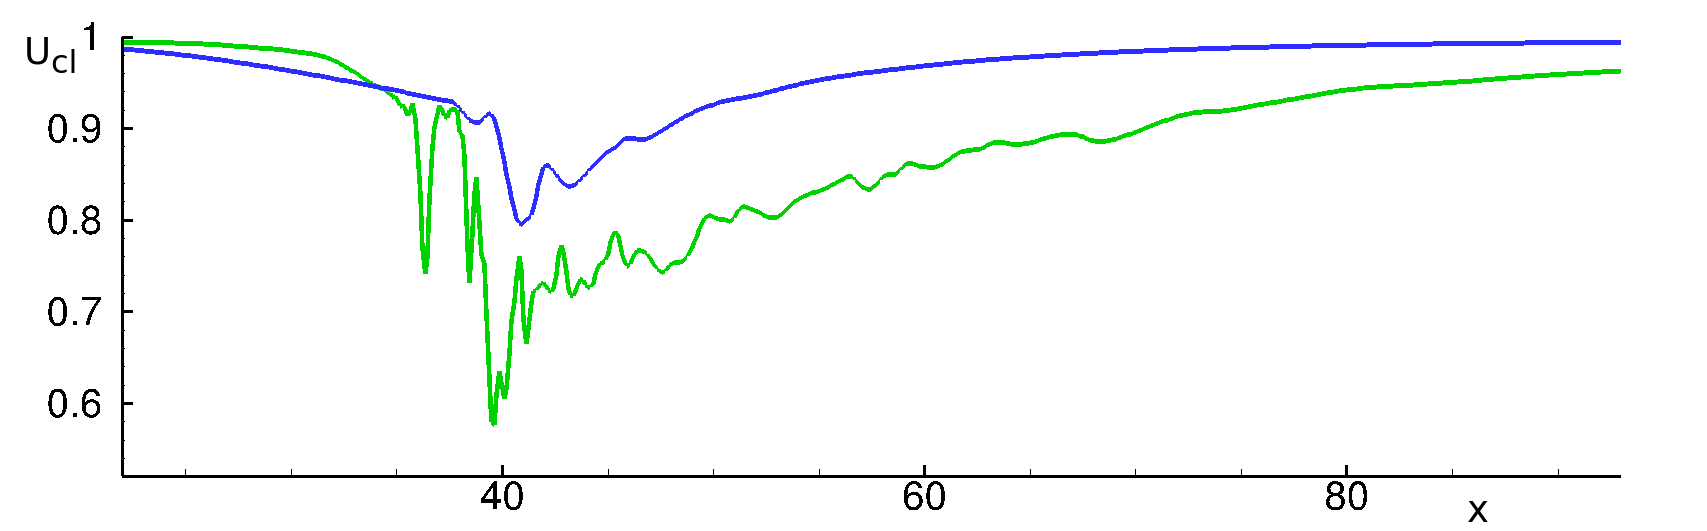
\includegraphics[width=1\linewidth]{ucl_cmp.png}}
\caption{Сравнение скорости на оси трубы $U_cl$ в турбулентном порыв (зеленая линия) и в модельном порыве (синяя линия).}
\label{ucl_cmp_img}
\end{figure}

\section{Свойства модельного порыва}

Для удобства перейдем в подвижную систему координат, перемещающуюся вдоль трубы со скоростью сноса локализованной структуры $C_f$. В подвижной системе решение представляется в виде суперпозиции стационарной составляющей $\u_s(\x)$ и колебательной $\u_n(t,\x)$. Стационарную составляющую в свою очередь представим в виде суперпозиции осесимметричной $\u_{2D}(\x)$ и трехмерной $\u_{3D}(\x)=\u_s-\u_{2D}$ составляющих. Распределения продольной компоненты осесимметричной составляющей скорости вдоль трубы $u_{x,2D}(x)$ для нескольких расстояний от оси трубы представлены на фиг.~4,а (даны отклонения от течения Пуазейля). Начало системы отсчета $x=0$ помещено в сечение, в котором среднее отклонение скорости от течения Пуазейля максимально. Голова структуры, где начинает проявляться отклонение осевой скорости, располагается на расстоянии $x\approx45$. Хвостовая часть структуры на сепаратрисе очерчена не так четко, как в турбулентных порывах, где восстановление скорости происходит на отрезке длиной в $3-5$ радиусов трубы.  Падение скорости в приосевой области трубы компенсируется ускорением у стенки. Поведение радиальной компоненты $u_{r,2D}$, показанное на фиг.~4,б соответствует изменению осевой скорости --- в зоне замедления на оси происходит растекание жидкости к стенкам, $u_{r,2D}>0$, в передней части происходит обратный процесс и $u_{r,2D}<0$.

На фиг.~5 приведены распределения по $x$ среднеквадратичных по сечению трубы амплитуд трех составляющих движения: стационарной осесимметричной (отклонение от течения Пуазейля) $A_{2D}$, стационарной трехмерной $A_{3D}$ и колебательной $A_n$. Распределение $A_{2D}(x)$ соответствует фиг.~4. Отклонение от течения Пуазейля заметно на значительном отрезке от $x=-30$ до $x=40$. Максимум $A_{2D}$ составляет  8.4\%. Величина $A_{3D}$ характеризует интенсивность полосчатых структур. Как видно на фиг.~2 полосчатые структуры появляются на некотором расстоянии вверх по потоку от головы порыва и сохраняются на значительном расстоянии позади него. В согласии с этим $A_{3D}(x)$ имеет выраженную асимметрию относительно точки $x=-2$, где эта величина достигает максимума. Интенсивность полос быстро падает вниз по потоку и сохраняется на значительном расстоянии в верхней части потока. В отличие от стационарных полосчатых структур, колебательная составляющая движения сосредоточена на сравнительно непротяженном отрезке трубы от $x=-5$ до $x=15$ с максимальной амплитудой в 4\% при $x=2.5$.

\section{Механизм самоподдержания модельного порыва} 

Все описанные составляющие движения находятся в динамическом взаимодействии друг с другом. Как видно на рис.~5 наиболее локализованной вдоль трубы оказывается колебательная составляющая. Распределения среднеквадратичной амплитуды колебаний в нескольких сечениях трубы приведены на фиг.~6. Мгновенные колебания в соответствии с условием (\ref{per}) распределены по углу с периодом $\pi$, при этом колебания в точках $(x,r,\theta)$ и $(x,r,\pi/2\pm\theta)$ совпадают со сдвигом на полпериода по времени. Этим объясняется угловая $\pi/2$-периодичность амплитуды колебаний. Доминирующая мода колебательной составляющей пропорциональна $\exp(2\pi it/T)$ во времени и $\exp(2i\theta)$ в угловом направлении. Нелинейное взаимодействие колебательных мод порождает колебания на высших частотах, а также дает вклад в стационарную составляющую движения. В стационарной составляющей кроме осесимметричной части доминирует мода, пропорциональная $\exp(4i\theta)$, то есть с периодом $\pi/2$ в угловом направлении. Именно такой периодичности по углу соответствуют четыре пары полосчатых структур, наблюдающихся при решении задачи с условиями (\ref{sym}),(\ref{per}).

Отметим, что непосредственный вклад колебаний в образование полос не велик. Основной механизм роста полос это так называемый лифтап (lift-up) эффект, связанный с появлением движения в перпендикулярной к основному потоку плоскости. Частицы жидкости, перемещающиеся от стенки в сторону оси трубы, приносят дефект скорости и образуют полосу замедления, а частицы двигающиеся в противоположном направлении --- от оси к стенке, образуют полосу ускорения. Основная роль колебательной составляющей в этом механизме состоит именно в порождении стационарного движения в поперечной плоскости, распределение среднеквадратичной амплитуды которого $A_\bot(x)$ также представлено на фиг.~5. Как видно, область сосредоточения поперечного движения практически совпадает с областью существования колебаний. Некоторое уклонение $A_\bot(x)$ в заднюю сторону объясняется конвективным переносом этого движения (поперечное движение в основном возникает в периферийной части сечения трубы, где скорость потока в выбранной системе отсчета отрицательна).

Стационарное поперечное движение направлено от оси трубы к стенке в областях $\theta=k\pi/2$ и наоборот, от стенки к оси в промежуточных областях $\theta=\pi/4+k\pi/2$. Соответственно, в первых возникают полосы ускорения, во вторых --- замедления. Распределения скорости полосчатых структур в нескольких сечениях трубы приведены на фиг.~7. В сечении $x=0$, где максимальна (среди сечений, представленных на фиг.~7) интенсивность поперечного движения, изображено также векторное поле поперечного движения, демонстрирующее лифтап механизм образования полосчатых структур. На всех сечениях фиг.~7 сплошной линией изображена линия нулевой скорости осесимметричной составляющей движения в подвижной системе отсчета. В приосевой области, ограниченной этой линией, скорость положительна, а в периферийной --- отрицательна. Как видно из рисунков, полосчатые структуры во всех сечениях кроме самого переднего из представленных ($x=5$) располагаются в области отрицательной относительной скорости. Осесимметричное движение с отрицательной скоростью переносит полосчатые структуры в заднюю часть порыва, где они формируют картину, похожую на вытянутые щупальса медузы (см. фиг.~2). При $x>5$ полосчатые структуры концентрируются в приосевой части трубы и конвектируются вперед положительной скоростью относительного движения, благодаря чему в передней части порыва $A_{3D}$ сохраняет заметную величину, несмотря на отсутствие поперечного движения.

Полосчатые структуры достигают максимальной своей амплитуды в области $x\in[-5,0]$, где создаются условия для возникновения колебаний. Наиболее вероятный механизм генерации колебаний --- механизм потери устойчивости стационарной составляющей течения. Для проверки этой гипотезы стационарное течение с полем скорости $\u_s$ было исследовано на устойчивость к малым возмущениям. Линеаризованные относительно возмущений уравнения с некоторыми случайными начальными условиями интегрировались по времени до выхода решения на режим экспоненциального изменения. Обнаружено, что действительно поле скорости $\u_s$ неустойчиво к малым возмущениям. Растущее возмущение $\sim\exp(\lambda+i\omega)t$ имеет коэффициент роста $\lambda=0.012$ и частоту $\omega=0.116$, близкую к частоте колебаний $2\pi/60=0.105$ в решении на сепаратрисе. Что еще более существенно, распределение амплитуды колебаний в растущем решении задачи линейной устойчивости оказывается близким к соответствующим распределениям колебательной составляющей решения на сепаратрисе. Таким образом, нет сомнений, что механизмом появления колебаний является линейная неустойчивость стационарной составляющей движения.

Отметим, что неустойчивость полосчатых структур является неотъемлемой составляющей всех сценариев самоподдержания турбулентности в пристенных течениях. При этом чаще всего предполагается, что неустойчивость возникает в пристенных областях полос замедленного движения, где в локальном профиле скорости $U(r)$ на фоне наибольшего градиента появляется точка перегиба --- источник неустойчивости в механизме типа Кельвина--Гельмгольца. В частности, именно такой механизм предлагается в качестве механизма возникновения колебаний в турбулентном порыве в [11]. В рассматриваемом нами решении на сепаратрисе это определенно не так. Как видно на фиг.~6 в сечении $x=0$, соответствующем максимальной скорости роста колебаний, амплитуда колебаний минимальна как раз в области полосы замедления ($\theta=\pi/4$). Наибольшие колебания развиваются наоборот вблизи полос ускорения, а если быть более точным, в промежуточных областях между полосами. В этих областях стационарная составляющая скорости течения претерпевает наибольшее изменение и имеет точки перегиба, но не как функция радиальной переменной, а как функция угла. Во всех сечениях фиг.~6 сплошными линиями изображены линии нулевой относительной скорости стационарной составляющей течения. Видно, что в сечении $x=0$, где происходит основной рост колебаний, в областях максимальной амплитуды колебаний наблюдается наиболее быстрое изменение скорости как функции угловой переменной.

Отметим также, что точки максимального роста колебаний находятся на линии $r\approx0.4$, что соответствует нулевой относительной скорости. По этой причине область порождения колебаний остается неподвижной относительно порыва. Интересно, что в этой же области ($x=0,\ r\approx0.4$) происходит смена знака радиальной компоненты осесимметричной составляющей скорости (см. фиг.~4,б). При $x<0$ радиальная скорость положительна, поэтому колебания, возникшие в задней части порыва, относятся в сторону стенки трубы, где относительная скорость отрицательна, и уносятся в хвостовую часть порыва. Наоборот, при $x>0$ радиальная скорость направлена к оси трубы, туда же, в область положительной скорости, сносятся и колебания, обнаруживающиеся в передней части порыва.


\section{Бегущая волна}


\section{Механизм образования продольных вихрей.}

Продольные вихри в стационарной составляющей движения возникают в результате нелинейного взаимодействия пульсаций. Это, в частности, подтверждается фактом совпадения областей концентрации продольных вихрей и пульсаций вдоль трубы. Прояснить процесс формирования продольных вихрей позволяет анализ уравнения, описывающего эволюцию продольной завихренности, полученного применением оператора Ротора к уравнению Навье-Стокса \eqref{NSeq_cf}:
\begin{equation}\label{ox_eq}
\pd{\omega_x}{t} - \nu\nabla^2 \omega_x =  -  (\v - \c_f, \nabla) \omega_x + (\om, \nabla) v_x
\end{equation}
Здесь $\om = (\omega_x, \omega_r, \omega_\theta) = \rot \v$ --- вектор завихренности, $\c_f$ --- скорость перемещения системы отсчета. Уравнение для стационарной составляющей продольной завихренности получается после осреднения \eqref{ox_eq} по времени в системе отсчета, связанной с порывом:
\begin{equation}\label{OX_eq}
\pd{\Omega_x}{t} - \nu\nabla^2 \Omega_x = - (\V - \c_f, \nabla) \Omega_x + (\Om, \nabla) V_x - \overline{(\v', \nabla) \omega'_x}^t + \overline{ (\om', \nabla) v'_x }^t
\end{equation}
Здесь  $\Om=(\Omega_x, \Omega_r, \Omega_\theta)$ и $\om'=(\omega'_x, \omega'_r, \omega'_\theta)$ средняя и пульсационная составляющие вектора завихренности. Черта над выражением --- знак осреднения по переменной, указанной верхним индексом. В правой части \eqref{OX_eq} первая пара членов описывает изменение продольной завихренности за счет конвективного переноса и деформации вихревых линий осредненного течения, а вторая пара выражает порождение средней завихренности пульсационным движением. При отсутствии пульсаций продольная завихренность постепенно исчезает под действием вязкости. В рассматриваемом течении система находится в равновесии и стационарная продольная завихренность во времени не меняется. Вязкие диссипация и диффузия компенсируются генерацией завихренности членами в правой части \eqref{OX_eq}.

Для выявления определяющих механизмов генерации средней продольной завихренности удобнее рассмотреть уравнение эволюции квадрата $\Omega_x$, получающееся домножением всех членов \eqref{OX_eq} на $2\Omega_x$. Положительный или отрицательный знак у полученных таким образом выражений в правой части уравнения показывает соответственно положительный или отрицательный вклад этого члена в изменение $\Omega_x^2$, а, следовательно, и в интенсивности поперечного движения. Распределение $\Omega_x^2$ по сечению трубы представлено на рис.~\ref{OXgen_pic}(a). В большей части сечения трубы средняя продольная завихренность близка к нулю. Область концентрации $\Omega_x$ расположена между полосами повышенной и пониженной скорости вблизи области максимальной амплитуды пульсаций.

\begin{figure}[h]
\center{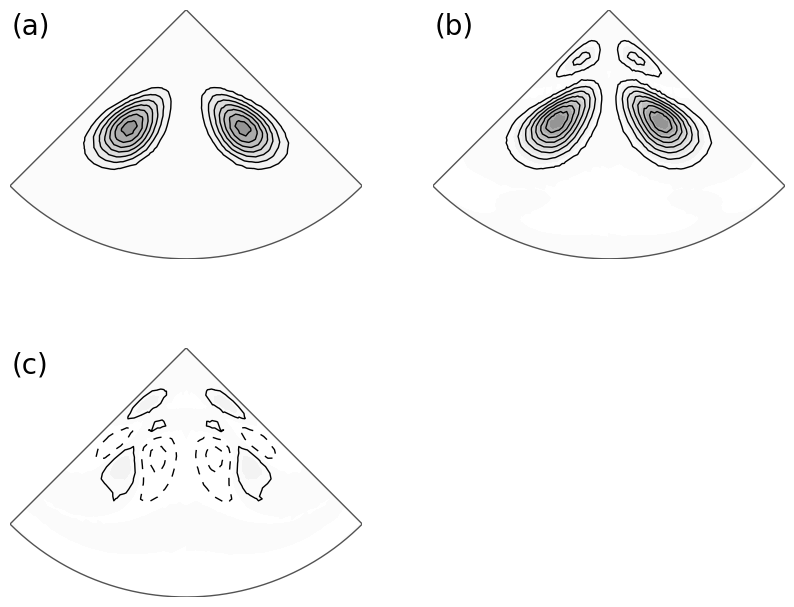
\includegraphics[width=0.9\linewidth]{OXgen.png}}
\caption{Распределение по сечению трубы $\Omega_x^2$ --- (a), вклад в производство $\Omega_x^2$ слагаемых, соответствующих выделенным в \eqref{OXgen_terms} --- (b), вклад остальных слагаемых в правой части \eqref{OX_eq} --- (с). Сплошные линии соответствуют положительным значениям, прерывистые --- отрицательным.}
\label{OXgen_pic}
\end{figure}

При анализе уравнения \eqref{OX_eq} обнаружено, что два слагаемых в правой части, а именно
\begin{equation}\label{OXgen_terms}
 - \overline{v'_x \frac{\d \omega'_x}{\d x}} + \overline{ \omega'_x \frac{\d v'_x}{\d x} },
\end{equation}
вносят определяющий вклад в производство средней продольной завихренности. Соответствующее сумме \eqref{OXgen_terms}  распределение в уравнении для $\Omega_x^2$ представлено на рис.~\ref{OXgen_pic}(b), а вклад остальных слагаемых правой части \eqref{OX_eq} показан на рис.~\ref{OXgen_pic}(c). Распределение генерации $\Omega_x^2$ выделенными в \eqref{OXgen_terms} членами практически совпадает по форме с распределением $\Omega_x^2$, тогда как вклад остальных членов не имеет выраженного распределения и более чем на порядок уступает по суммарному вкладу в генерацию $\Omega_x^2$. Таким образом, нет сомнения в том, что стационарные продольные вихри возникают в основном за счет действия выделенной в \eqref{OXgen_terms} пары слагаемых.

Отметим, что пульсации, соответствующие старшей собственной функции линейной задачи об устойчивости среднего стационарного течения, также демонстрируют приведенный выше механизм образования стационарных продольных вихрей. Важно, что это наблюдается только в том случае, когда при анализе устойчивости учитываются как продольная, так и поперечная составляющие среднего течения. Принято считать, что поперечное движение, определяя угловую неоднородность в распределении продольной скорости среднего течения, не может существенным образом влиять на свойства его устойчивости вследствие незначительности своей амплитуды. Поэтому при исследовании линейной устойчивости подобных течений, например, полосчатых структур в турбулентных потоках, наличие поперечного движения обычно не принимается во внимание. В нашем случае пренебрежение поперечным движением приводит к тому, что стационарное течение оказывается линейно устойчивым. Что еще более важно, наименее затухающее возмущение не воспроизводит при этом описанный механизм формирования продольных вихрей. Это связанно с тем, что форма пульсаций продольной завихренности $\omega'_x$ качественно меняется, хотя пульсации продольной скорости $v'_x$ сохраняют свою форму практически неизменной. Тем самым нарушается согласованность  $v'_x$ и $\omega'_x$, необходимая для обеспечения нужного вклада выражения \eqref{OXgen_terms} в производство продольной завихренности.

Каждое из двух слагаемых в \eqref{OXgen_terms} дает примерно половину общего вклада в производство средней продольной завихренности. Это значит, в частности, что колебания $\d v'_x/\d x$ и $\omega'_x$ положительно коррелированы в области концентрации положительной $\Omega_x$ и отрицательно коррелированы в области концентрации отрицательной $\Omega_x$. То же относится и к колебаниям $-v'_x$ и $\d \omega'_x/\d x$. Расчет соответствующих коэффициентов корреляции показывает, что они близки к $\pm1$ в соответствующих областях. 


\section{Механизм возникновения пульсаций продольной завихренности}

Для выявления механизма формирования такой связи между пульсациями продольных компонент скорости и завихренности рассмотрим уравнение эволюции $\omega'_x$, получающееся вычитанием \eqref{OX_eq} из \eqref{ox_eq}:
\begin{multline}\label{ox1_eq}
\pd{\omega'_x}{t} - \nu \nabla^2 \omega'_x = - (\V - \c, \nabla) \omega'_x - (\v', \nabla) \Omega_x
+(\Om, \nabla) v'_x + (\om', \nabla) V_x -\\- (\v', \nabla) \omega'_x  + (\om', \nabla) v'_x  + \overline{(\v', \nabla) \omega'_x)}  - \overline{(\om', \nabla)}
\end{multline}
Работать удобнее с уравнением, описывающим изменение среднего квадрата пульсаций продольной завихренности $\overline{\omega'^2_x}$, получающимся умножением на $2\omega'_x$ каждого из слагаемых в \eqref{ox1_eq} и последующим осреднением по времени. Как и раньше, осреднение по времени производится в подвижной системе отсчета. Слагаемые в этом уравнении не зависят от времени, сумма слагаемых в правой части балансируется вязким членом в левой части. Как и в предыдущем случае, среди всех слагаемых правой части удается выделить существенные, ответственные за возникновение пульсаций $\omega'_x$.


Распределение $\overline{\omega'^2_x}$ по сечению трубы с максимальным уровнем пульсаций изображено на рис.~\ref{ox1gen_pic}(a). Основные пульсации $\omega'_x$ наблюдаются в центре расчетной области около оси трубы. На месте расположения продольных вихрей также присутствуют пульсации $\omega'_x$, но меньшей интенсивности. В остальной части трубы их амплитуда близка к нулю. Обнаружено, что за генерацию пульсаций $\omega'_x$ в центральной части трубы и на месте продольных вихрей отвечают два разных механизма. Первый дает пульсации большей амплитуды, однако, за возникновение стационарных продольных вихрей ответственны пульсации, производимые вторым механизмом, так как именно они оказываются согласованными с пульсациями $v'_x$ нужным образом.


\begin{figure}[h]
\center{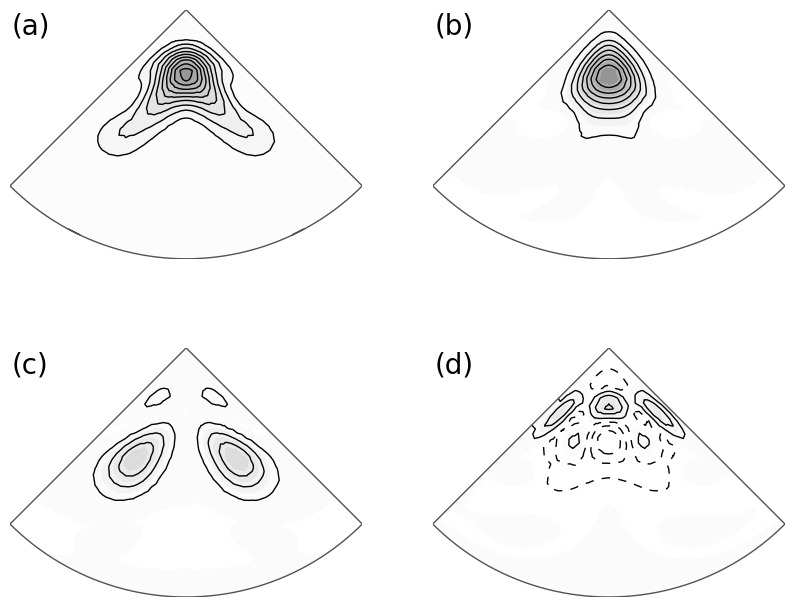
\includegraphics[width=0.9\linewidth]{ox1gen.png}}
\caption{Распределение среднего квадрата пульсаций продольной завихренности --- а, вклад в производство $\left<\omega'^2_x \right>$ слагаемых \eqref{ox1gen_add_terms} --- (b), слагаемого \eqref{ox1gen_main_terms} --- (c) и суммы остальных слагаемых правой части \eqref{ox1_eq} --- (d).}
\label{ox1gen_pic}
\end{figure}


Первый механизм формирования $\omega'_x$ связан с наличием нормальных к стенке вихрей в пульсационной составляющей движения. Можно провести аналогию между неустойчивостью, возникающей на полосе замедления, и неустойчивостью в следе за телом. Пульсационная составляющая движения напоминает дорожку Кармана. В ней можно выделить последовательность нормальных к стенке вихрей чередующегося знака, двигающихся вниз по полосе пониженной скорости. Им соответствуют области повышенной амплитуды пульсаций радиальной завихренности $\omega'_r$. Между полосой замедления и осью трубы имеется значительный радиальный градиент продольной скорости $\d V_x/ \d r$. В его присутствии нормальные к стенке вихри поворачиваются так, что приобретают продольную составляющую $\omega'_x$. Кроме того, наличие радиального градиента $\d V_x/ \d r$ связано с наличием угловой завихренности $\Omega_\theta = \d V_r / \d x - \d V_x / \d r$. Радиальная пульсационная завихренность $\omega'_r = \d v'_x / r \d \theta - \d v'_\theta / \d x$ за счет первого из слагаемых поворачивает стационарные угловые вихри так, что те также приобретают пульсационную продольную составляющую. В уравнении \eqref{ox1_eq} за описанный механизм отвечают слагаемые:
\begin{equation}\label{ox1gen_add_terms}
\frac{\d \omega'_x}{\d t} = \omega'_r \frac {\d V_x}{\d r} +
\frac{\Omega_\theta}{r} \frac{\d v'_x}{\d \theta} + ...
\end{equation}
Несмотря на то, что выделенные в \eqref{ox1gen_add_terms} слагаемые имеют противоположные знаки и в значительной степени компенсируют друг друга при сложении, их вклад в производство $\omega'_x$ значителен (см. рис.~\ref{ox1gen_pic}(b)). Они определяют форму пульсаций $\omega'_x$ в области между полосой замедления и осью трубы, где пульсации $\omega'_x$ достигают наибольшего значения. Эти пульсации, однако, практически не участвуют в образовании стационарной составляющей продольной завихренности. Это объясняется тем, что колебания $\omega'_x$, рождающиеся в результате описанного механизма, близки по фазе к колебаниям $v'_x$, так что сомножители каждого из слагаемых в выражении \eqref{OXgen_terms} оказываются в противофазе и при осреднении дают близкие к нулю значения.


Второй механизм образования пульсаций продольной завихренности $\omega'_x$ связан с перераспределением уже существующей стационарной продольной завихренности $\Omega_x$ за счет пульсационной составляющей продольной скорости $v'_x$ (эффект сжатия/растяжения вихревых линий). В уравнении \eqref{ox1_eq} за описываемый механизм отвечает слагаемое
\begin{equation}\label{ox1gen_main_terms}
\frac{\d \omega'_x}{\d t} = \Omega_x \frac {\d v'_x}{\d x} + ...
\end{equation}
Выделенное в \eqref{ox1gen_main_terms} слагаемое стремится произвести пульсации $\omega'_x$, пропорциональные $\d v'_x / \d x$, что обеспечивает наибольшую эффективность образования $\Omega_x$ посредством их нелинейного взаимодействия. Важно, что коэффициентом пропорциональности в \eqref{ox1gen_main_terms} выступает значение средней продольной завихренности, таким образом, механизм включается именно в областях концентрации $\Omega_x$. При этом производимые пульсации $\omega'_x$ положительно пропорциональны пульсациям  $\d v'_x / \d x$ при $\Omega_x>0$ и отрицательно пропорциональны при $\Omega_x<0$, что обеспечивает максимально возможную эффективность производства средней продольной завихренности нужного знака посредством второго из слагаемых выражения \eqref{OXgen_terms}. Очевидно, что пульсации $-v'_x$ и $\d \omega'_x / \d x$ в этом случае также согласованы нужным образом, так что первое слагаемое \eqref{OXgen_terms} близко по значению ко второму.


На рис.~\ref{ox1gen_pic}(c) приведен вклад выделенного в \eqref{ox1gen_main_terms} слагаемого в производство $\overline{\omega'^2_x}$. Нет сомнения, что именно это слагаемое определяет форму пульсаций в области существования продольных вихрей между полосами повышенной и пониженной скорости. Суммарный вклад других слагаемых правой части \eqref{ox1_eq}, не попавших на рис.~\ref{ox1gen_pic}(b,c), изображен на рис.~\ref{ox1gen_pic}(d). Эти слагаемые не имеют существенного значения в процессе генерации $\omega'_x$, их суммарный вклад не превышает нескольких процентов.

Описанный механизм генерации пульсаций продольной завихренности проявляется в области, где фазовая скорость волны, соответствующей пульсационной составляющей течения, близка по значению к локальной продольной скорости среднего течения. На удалении от точки генерации пульсаций, где фазовая скорость волны существенно отличается от средней скорости, выделенный в \eqref{ox1gen_main_terms} механизм генерации $\omega'_x$ практически не работает. Это объясняется тем, что в системе отсчета, связанной с волной, образующаяся посредством механизма \eqref{ox1gen_main_terms} $\omega'_x$ сносится вдоль трубы средним течением. При этом теряется согласованность фаз между $\d v'_x / \d x$ и $\omega'_x$, что делает её рост невозможным.


Описанный механизм генерации пульсаций продольной завихренности объясняет необходимость учета поперечного движения при исследовании устойчивости стационарного течения. Пренебрежение связанной с поперечным движением $\Omega_x$ делает невозможным генерацию $\omega'_x$ в форме, необходимой для сохранения поперечного движения, а следовательно и всего процесса самоподдержания пульсаций.



\chapter{}

В предыдущей главе, исследуя модельный порыв, удалось получить некоторые представления о его структуре и механизме самоподдержания. В настоящей главе поднимается вопрос об общности полученных результатов. Тот факт, что продольные вихри и пристенные полосы присутствуют как в других инвариантных решениях \cite{Kawahara2012}, так и в пристенной турбулентности \cite{Kline1967, Smith1983, Schoppa2002}, позволяет предполагать, что выделенный механизм генерации пульсаций может быть частично или полностью обобщен на эти случаи. Выполнить строгое исследование турбулентного течения сегодня не представляется возможным, однако полученные результаты могут быть проверены на других инвариантны решения. Опираясь на модельный порыв метод продления в пространстве параметров \cite{Sanchez2004, Viswanath2007, Dijkstra2014} позволяет получить новые локализованные в пространстве инвариантные решения. Среди них могут быть выделены такие, характеристики которых ближе к наблюдаемым в турбулентном течении, что повышает ценность полученных при их исследовании результатов. 

%\begin{comment}
Все периодические решения удовлетворяют нелинейному уравнению вида
$$
\v_p = \phi(\v_p, T, c_p, Re).
$$ 
Функция $\phi(\v, t, c, \Re)$ возвращает поле скорости, возникающее в результате эволюции поля скорости $\v$ в течении времени $t$ при числе Рейнольдса $\Re$ в системе отсчета, двигающейся со скоростью $\c$. $\v_p$, $T$ и $c_s$ --- подлежащие определению поле скорости периодического решения, его период во времени и скорость перемещения вдоль трубы.
%\end{omment}
Все периодические решения удовлетворяют нелинейному уравнению, которое может быть решено методом Ньютона, обобщенным на случай многих неизвестных, называемым также методом Ньютона-Рафсона \cite{}. Метод Ньютона итерационный и требует начального приближения из некоторой окрестности решения. С произвольным начальным приближением метод не сходится, основная сложности в поиске инвариантных решений сводится к нахождению подходящего начального приближения. Однако, если хотя бы одно решение известно, оно может выступать в качестве начального приближения к решению с близким значением параметров, в частности, числа Рейнольдса, с которым метод сойдется. Таким образом, решение может быть продлено в сторону увеличения или уменьшения числа Рейнольдса. В пространстве $(T, c_f, \Re)$ решение принадлежит однопараметрическому множеству. Следуя работе \cite{Avila2013}, продлевая модельный порыв в сторону уменьшения числа Рейнольдса, при $\Re_{biff} = $ удалось достичь точки бифуркации (В \cite{Avila2013} сообщается о $\Re_{biff} = $), в которой возникает две ветви решения, и перейти с нижней ветви решения на верхнюю. Верхняя ветвь решения характеризуется более высокой интенсивностью пульсаций и меньшей скоростью сноса, чем нижняя, что приближает характеристики решения к турбулентному течению. Если нижняя ветвь решения находится на границе турбулентного бассейна притяжения, так как принадлежит сепаратрисе, верхняя ветвь решения находится внутри турбулентного бассейна притяжения, и возможно участвует в формировании турбулентного аттрактора. 

Исследуя решение с верхней ветви удалось показать, что его структура и механизм самоподдержания аналогичны структуре решения с нижней ветви, что подтверждает общий характер выделенных механизмов. Хотя решение с верхней ветви связано с решение с нижней непрерывным образом, и качественно их механизм поддержания отличаться не может, выделенный механизм мог оказаться неприменим к верхней ветви, если бы был неверно формализовано.

На каждом шаге метода Ньютона-Рафсона возникает необходимость решения матрицы Якоби. В случае задач вычислительной гидродинамики, где число неизвестных достигает миллионов, формирование и даже хранение матрицы Якоби в явном виде невозможно, так как число элементов в ней составляет квадрат числа неизвестных в уравнении. Используя Крыловские методы для решения матрицы Якоби удается радикальным образом сократить число операций и необходимой оперативной памяти, что делает расчеты возможными. В работе реализован метод Ньютона-Крылова \cite{}, основанный на методе GMRES (generalized minimum residual method) \cite{Saad1986}. Альтернативой методу GMRES может быть метод BiCGSTAB (Biconjugate gradient stabilized method) \cite{Sleijpen1993}. 

В континуальной постановке не формулируется. 

\section{Продление решений в пространстве параметров}

Решение поставленной задачи $\v_p(x,r,\theta,t)$ является периодическим по времени с периодом $T$, если оно удовлетворяет условию
\begin{equation} \label{tper_eq}
\v_p(x,r,\theta,t) = \v_p(x - c_p T, r, \theta, t + T),
\end{equation}
Однородность наложенных условий вдоль трубы рождает возможность смещения решения в этом направлении. Как следствие, в условии \eqref{tper_eq} возникает параметр $c_p$, определяющий скорость сноса решения вдоль оси $x$. Возможность смещения решения в угловом направлении исключена дополнительным условием отражения относительно плоскости $\theta = 0$ \eqref{sym_eq}. В отсутствии условия \eqref{sym_eq} также возник бы параметр, отвечающий за возможный поворот решения вокруг оси трубы. По сути, возможность существования периодического по времени решения со свободным параметром $T$ является следствие однородности граничных условий по $t$. 

В конечно-разностной постановке условие периодичности по времени может быть сформулировано иначе
\begin{equation}\label{P_eq}
\phi(\v_p, T, c_p, \Re, \dots) - \v_p = 0.
\end{equation}
Здесь функция $\phi(\v, t, c, \Re, \dots)$ возвращает поле скорости, возникающее в результате эволюции поля скорости $\v$ в течении времени $t$ при числе Рейнольдса $\Re$ в системе отсчета, двигающейся со скоростью $c$. В число параметров функции $\phi$ могут входить также и другие величины, такие как длина периода вдоль трубы $L_x$ или длина периода в угловом направлении $2\pi/n$, если полагать, что $n$ может принимать действительные значения. С практической точки зрения, вычисление функции $\phi$ требует численного интегрирования поля скорости $\v$ по времени. 

Периодические решения обладают двумя непрерывными симметриями. Решение остается решение при смещении вдоль трубы на произвольное расстояние и при смещении по времени на произвольную величину. Для того, чтобы уравнение \eqref{P_eq} имело однозначное решение, необходимо исключить возможность смещения решения вдоль трубы и во времени. Для этого на поле скорости $\v_p$ накладывается пара дополнительных условий вида 
\begin{equation}\label{Pplus_eq}
r_{1,2}(\v_p) = 0.
\end{equation}
В этом случае, если поле скорости однозначно задается $N$ переменными, то количество уравнений в системе равно $N+2$. Для того, чтобы число неизвестных в системе совпадало с числом уравнений, необходимо вместе с полем скорости $\v_p$ положить неизвестными два параметра системы. В случае, если решение ищется при фиксированном значении $\Re$ на заданной сетке, это могу быть $T$ и $c_p$. 

Система \eqref{P_eq}, \eqref{Pplus_eq} может быть представлена в виде 
\begin{equation}\label{F_eq}
F(\x) = 0, 
\end{equation}
где вектор $\x = (\v_p, T, c_p, \Re, \dots)$ объединяет все переменные системы. Рассмотрим её полный дифференциал
\begin{equation}\label{dF_eq}
dF = \pd{F}{\x}d\x.
\end{equation}
В случае, если фиксированы все параметры кроме трех, например $(T, c_p, \Re)$, Якобиан ${\d F}/{\d \x}$ оказывается прямоугольной матрицей, содержащей $(N+2)$ строк и $(N+3)$ столбцов, система \eqref{dF_eq} недоопределена. В этом случае в окрестности каждого решения существует направление $d\x_0$, для которого $dF = 0$, при движении вдоль которого решение остается решением, так как значение $F$ сохраняется равным нулю. Тогда решения в пространстве трех параметров принадлежат некоторой кривой, задаваемой одним параметром $\x_p = \Gamma(s)$, полученной интегрирование вдоль направления $d\x_0$. Аналогично, в пространстве четырех параметров решения принадлежат двухпараметрическому семейству, и т.д. Точки, где Якобиан имеет не полный ранг, могут быть точками бифуркации, в которой могут сходиться несколько ветвей решения \cite{Sanchez2004}. 

Таким образом, периодическое по времени решение, найденное в предыдущей главе, может быть продлено как в сторону увеличения, так и в сторону уменьшения числа Рейнольдса. Естественно параметры расчетной области положить фиксированными, а в качестве определяемых выбрать период решения по времени $T$ и скорость его перемещения вдоль трубы $c_p$. В пространстве параметров $(T, c_p, \Re)$ решения принадлежат некоторой кривой. Двигаясь по ней в сторону уменьшения $\Re$, удается достичь точки бифуркации, в которой решение возникает (При меньших $\Re$ оно не существует). В этой точке кривая, которой принадлежат решения, совершает разворот так, что в сторону увеличения $\Re$ направлено две ветви решения. Их называют нижней и верхней ветвью решения, причем исходное решение принадлежит нижней ветви. В точке бифуркации удается перейти на верхнюю ветвь решения, двигаясь по которой в сторону увеличения $\Re$, можно получить новое решение при исходном значении $\Re$. На каждой ветви число Рейнольдса однозначно определяет решение. 

Дополнительно можно отметить, что вместо условия периодичности по времени \eqref{tper_eq} может быть применено условие отражения относительно плоскости $\theta = 0$ со сдвигом на половину периода по времени $T/2$, которое выполнено для модельного порыва. Условие имеет вид
\begin{equation}\label{shift_eq}
\v_p(x,r,\pi/4 + \theta,t) = \v_p(x - c_p T/2,r,\pi/4 - \theta,t+T/2).
\end{equation}
В этом случае уравнение \eqref{P_eq} уступит место следующему
\begin{equation}\label{P2_eq}
\v_p(x,r,\pi/4 - \theta) = \phi(\v_p, T/2, c_p, \Re, \dots)(x,r,\pi/4 + \theta).
\end{equation}
Его вычисление требует вдвое меньше времени, что может быть существенно при проведении численного исследования. При решении исходной системы \eqref{P_eq} существует некоторая вероятность потерять симметрию \eqref{shift_eq} в процессе продления решения, что исключено при решении системы \eqref{P2_eq}.


\section{Метод Ньютона-Крылова}

Система уравнений \eqref{F_eq} может быть решена численно методом Ньютона, обобщенным на многомерный случай, называемым также методом Ньютона-Рафсона. Метод ньютона итерационный и на каждом шаге уточняет существующее приближение к решению. Пусть $\x_m$ --- приближение к решению на шаге $m$, а $\x^*$ --- точное решение. Разложение выражения $F(\x^*)$ в ряд около точки $\x_m$ имеет вид
\begin{equation}
F(\x^*) = F(\x_m) + \pd{F}{\x}\bigg|_{\x_m} (\x^* - \x_m) + O(\Delta \x^2). 
\end{equation}
Пренебрегая малыми второго порядка, учитывая, что $F(\x^*) = 0$, получим линейную систему на поправку к решению $\Delta \x_m = \x_{m+1} - \x_m$
\begin{equation}\label{Newton_eq}
\pd{F}{\x}\bigg|_{\x_m} \Delta \x_m = - F(\x_m). 
\end{equation}
Основной задачей при применении метода Ньютона является решение системы \eqref{Newton_eq} и нахождение $\Delta \x_m$. Выполнение шага метода Ньютона завешается вычисление нового приближения к решению $\x_{m+1} = \x_m + \Delta x_m$. 


\def\l{\mathbf{l}}
В случае решения задач вычислительной гидродинамики размерность системы \eqref{Newton_eq} оказывается большой и может измеряться миллионами, её решение требует значительных вычислительных ресурсов. Еще более сложной задачей является формирование матрицы Якоби в явном виде. При поиске периодических решений привести аналитическое выражение для Якобиана не представляет возможным. для формирование матрицы Якоби пользуются тем фактом, что её произведение с произвольным вектором единичной длины $\l$ равно производной исходно функции $F$ вдоль этого направления
\begin{equation} \label{Jl_eq}
\pd{F}{\x} \l = \pd{F}{\l}. 
\end{equation}
Аналитическое вычисление производной функции $F$ в случае поиска периодических решений не представляется возможным. 
Она может быть получена численно, как конечная разность, по формуле
\begin{equation}\label{fd_eq}
\pd{F}{\l} \approx \frac{F(\x + \varepsilon \l) - F(\x)}{\varepsilon},
\end{equation}
при достаточно малом значении $\varepsilon$. В численных расчетах значение $\varepsilon$ рекомендуют выбирать порядка $10^{-7}$ \cite{Viswanath2007}. Вычисление матрицы Якоби сводится к вычислению производной функции $F$ вдоль каждого из базисных направлений, число которых равно числу неизвестных. В свою очередь, вычисление производной $F$ вдоль одного направления требует вычисления функции $F$ в новой точке. В случае поиска периодических решений при вызове функции $F$ выполняется численное интегрирование исходных уравнений в течении периода по времени, что требует значительны вычислительных затрат, и выполнить его $O(N)$ раз на практике невозможно. Даже хранение матрицы Якоби в памяти компьютера представляет серьезную вычислительную задачу.

Решить линейную систему \eqref{Newton_eq} позволяют итерационные методы, основанные на подпространствах Крылова. В этом случае обращение к матрице Якоби происходит только в форме её умножения на вектор, что следуя \eqref{fd_eq} сводится к вычислению конечно-разностной производной функции $F$ вдоль направления, задаваемого этим вектором. При решении системы вида 
\begin{equation}\label{Ax_eq}
Ax = b
\end{equation}
подпространство Крылова $K_i$ представляет собой линейную оболочку $i$ векторов
$$
K_i = L(b, Ab, A^2b, \dots, A^{i-1}b)
$$ 
Имея базис подпространства $K_i$, для того, чтобы построить базис в подпространстве $K_{i+1}$, необходимо выполнить только одно умножение матрицы $A$ на уже известный вектор $A^{i-1}b$. При решении системы \eqref{Ax_eq} приближение к решению ищется в базисе подпространства Крылова. Крыловские методы оказываются эффективны при поиске инвариантных решений с небольшим числом неустойчивых направлений (решение на сепаратрисе имеет одно неустойчивое направление \cite{}). Для уточнения решения на порядок требуется только несколько десятков базисных векторов в подпространстве Крылова. Таким образом, уточнение решения на порядок требует вычисления функции $F(\x)$ порядка $O(10)$ раз, число обращений к функции $F$ не зависит от размерности пространства $\x$. Метод Ньютона, в котором для решение линейной системы \eqref{Newton_eq} применяются методы Крыловского типа, называется также методом Ньютона-Крылова. 

\def\r{\mathbf{r}}
В работе был реализован основанный на подпространствах Крылова метод минимизации невязки \cite{EEbook}. Суть метода состоит в том, что на$i$-ой итерации в подпространстве $K_i$ ищется приближение к решению $\x_i$ таким образом, что длина невязки $\r_i = b - A\x_i$ в выбранной норме минимальна. Можно показать, что невязка имеет наименьшую длину в том и только том случае, когда она перпендикулярна пространству $AK_i$. Проще всего опустить перпендикуляр из вектора $b$ на подпространство $AK_i$, имея в этом подпространстве ортогональный базис. Построим последовательность векторов $q_1, \dots, q_i$ таким образом, что они образуют базис в подпространстве $K_i$, а вектора $p_1 = Aq_1, \dots, p_i = Aq_i$ образуют ортогональный базис в подпространстве $AK_i$. Тогда легко может быть построено ортоганальное разложение правой части уравнения вида $b = \alpha_1 p_1 + \dots + \alpha_i p_i + r_i$, где $b_i =  \alpha_1 p_1 + \dots + \alpha_i p_i$ лежит в пространстве $AK_i$, а $r_i$ перпендикулярно ему. Коэффициенты разложения дает формула
\begin{equation}
\alpha_k = (b,p_k) / (p_k, p_k),
\end{equation}
где $(\ ,\ )$ ---  скалярное произведение, порождающее норму, в которой минимизируется невязка. 
Так как у каждого вектора $p_k$ известен прообраз, линейна комбинация векторов $q_k$ с коэффициентами $\alpha_k$ дает приближение к решению, лежащее в пространстве $K_i$
\begin{equation}
\x_i = \alpha_1 q_i + \dots + \alpha_i q_i. 
\end{equation}
Переход на $i+1$ итерацию алгоритма связан с построением базиса подпространств $K_{i+1}$ и $AK_{i+1}$. Для построения ортогонального базиса в подпространстве $AK_{i+1}$ базис подпространства $AK_i$ пополняется новым вектором $p_{i+1}$, полученным ортогонализацией с уже известными базисными векторами $p_1, \dots, p_i$ вектора $Ap_i$. В процессе ортогонализации также может быть получен вектор $q_{i+1}$, являющийся прообразом вектора $p_{i+1}$. 

Критерием остановки итерационного процесса может служить снижение величины невязки ниже заранее заданного порогового значения, либо привышение заранее заданного числа итераций. Переход на новый шаг выполнения метода требует однократного вычисления произведения матрицы $A$ на вектор, связанного в применении к методу Ньютона с одним вычисление функции $F$. В процессе вычислений необходимо хранить две последовательности векторов $p_1, \dots, p_i$ и $q_1, \dots, q_i$. На первой итерации $q_1 = b$, $p_1 = Ab$. 

Метод Ньютона-Крылова может быть реализован поверх уже существующего кода без необходимости вносить в него изменения. 


\section{Реализация метода Ньютона-Крылова}

Незначительная модификация метода Ньютона Крылова позволяет решать систему $\eqref{P_eq}$ без дополнительных условий $\eqref{Pplus_eq}$ 


\section{Стратегия продления решения}

Реализованный метод Ньютона-Крылова позволяет находить периодические решения, но только в том случае, когда известно достаточно близкое к решению начальное приближение. С произвольными начальными данными метод Ньютона не сходится. В нашем случае в качестве начального приближения может выступать решение на сепаратрисе, найденное в предыдущей главе. Метод Ньютона-Крылова позволяет его уточнить, но кроме этого, оно может быть использовано в качестве начального приближения для решения с близкими значениями параметров, например, числа Рейнольдса. Если смещение по $\Re$ достаточно мало, метод Ньютона сходится, и дает новое периодическое решение. Таким образом, решение может быть продлено в пространстве параметров. Если уже получено несколько решений, приближение к новому может быть построено интерполяцией. В этой работе в основном применялась линейная интерполяция. Если $\x_1$ и $\x_2$ --- известные решения, полученные при числах Рейнольдса $\Re_1$ и $\Re_2$, то приближение к новому решению $\x_3$ при $\Re_3$ может быть получено по формуле 
\begin{equation}
\x_3 = \frac{\x_2(\Re_3 - \Re_1) - \x_1(\Re_3-\Re_2)}{\Re_2 - \Re_1}
\end{equation}

В случае, когда продвижение выполняется по $\Re$, а в качестве определяемых параметров выступают $T$ и $c_f$, преодолеть точку бифуркации и перейти с нижней ветви решения на верхнюю невозможно. Выполнить такой переход позволяет включение в число определяемых параметров $\Re$ вместо $T$ или $c_f$ на выбор. Другим методом решения может быть включение в число определяемых всех трех параметров $\Re$, $T$ и $c_f$. Как показывает практика, сходимость метода Ньютона при этом практически не меняется, хотя с формальной точки зрения она могла быть испорчена. Если в системе уравнений на периодическое решение \eqref{F_eq} неизвестных больше, чем уравнений, теряется однозначность решения. Линейная система для определения шага метода Ньютона \eqref{Newton_eq} получает бесконечно много решений произвольной длины. В процессе её решения может быть получено любое из них, и хотя оно является решением линейной системы, соответствующий ему шаг в пространстве $\x$ может вывести за пределы сходимости метода Ньютона. 

В более общем случае в пространстве параметров $(\Re, T, c_f)$ можно перейти к новой систем координат, одна из осей которой касается кривой $\Gamma(s)$, которой принадлежат решения. Пусть этой оси соответствует переменная $p_0$. Две другие оси, пусть $p_1$ и $p_2$, перпендикулярны оси $p_0$. При поиске нового решения имеет смысл фиксировать значение $p_0$, отделив тем самым новое решение от уже существующих. Тогда $p_1$ и $p_2$ выступают в качестве определяемых параметров и решение ищется в нормальной к кривой $\Gamma(s)$ плоскости. Получить приближение к направлению $p_0$ можно по уже известным решениям. Такой подход позволяет преодолеть точку бифуркации и другие особенности кривой $\Gamma(s)$ в автоматическом режиме. 

На нижней ветви вблизи решения, соответствующего модельному порыву, если в качестве начального приближения к новому решению выступает уже найденное, максимальный шаг по $\Re$ близок к $10$. При использовании линейной интерполяции, шаг может быть увеличен до величины порядка $100$. Хотя по мере продвижения в пространстве параметров шаг, с которым выполняется переход от уже найденного решения к новому, варьируется, можно выделить общую тенденцию, следуя которой по мере приближения к точке бифуркации допустимый шаг уменьшается. Хотя на верхней ветви решения допустимый шаг несколько увеличивается, он остается ниже, чем на нижней, ввиду большей сложности решения с верхней ветви. 
 









\chapter{Бегущие волны}
\section{Введение}
\section{Получение}
\section{Описание}
\section{Механизм самоподдержания}



\chapter{Заключение} 

Общепринято, что непременным атрибутом цикла самоподдержания турбулентности в пристенных течениях являются полосчатые структуры --- долгоживущие конечноамплитудные образования, возникающие в пристенных областях. Рассмотренные в данной работе пространственно-локализованные турбулентные порывы также обладают полосчатыми структурами, что свидетельствует о вероятной близости механизма их самоподдержания с механизмом самоподдержания однородной (нелокализованной) пристенной турбулентности. Изучено численное решение уравнений Навье--Стокса, аппроксимирующее течение в турбулентном порыве. Это предельное решение на сепаратрисе, разделяющей области притяжения ламинарного и турбулентного решений. Простота временного поведения этого решения позволяет провести исчерпывающее исследование механизма его самоподдержания. На рассмотренном примере подтверждена определяющая роль полосчатых структур. Наглядно показан процесс образования вытянутых полос, включающий действие лифтап  эффекта на ограниченном отрезке длины с последующим конвективным растяжением вдоль стенки трубы. Наиболее важный результат проведенного исследования состоит в том, что обнаруженная неустойчивость полосчатого движения противоречит общепринятой точке зрения, согласно которой доминирующей является неустойчивость Кельвина--Гельмгольца, возникающая в пристенных областях полос замедленного движения. В рассмотренном примере уровень колебаний в области полос замедления минимален. Генерация колебаний происходит в промежуточной области между полосами на фоне резкого изменения скорости вдоль угловой координаты. Для выяснения деталей механизма обнаруженной неустойчивости планируется более подробное исследование. Вопрос о степени приложимости сделанных выводов к течению в турбулентном порыве и другим турбулентным течениям остается за рамками данного исследования и находится в настоящее время в стадии изучения.

\newcommand{\listpub}{Список литературы}
\renewcommand{\bibname}{\listpub}

\phantomsection
\addcontentsline{toc}{chapter}{\tocsecindent{\listpub}}
\bibliography{bib/base,bib/rus,bib/books,bib/my}


\end{document}
